\section{Umsetzung}
\label{sec:realization}

Nachfolgend werden die
gemäss~\autoref{sec:description_implicit_surfaces} umgesetzten Konzepte
genauer beschrieben. Es handelt sich dabei um Ausschnitte des
umgesetzten Fragment-Shaders.

Das eigentliche Sphere Tracing geschieht in der Funktion
\textit{castRay}.  Diese hat als Parameter den Ursprung eines Strahles
(\textit{vec3 rayOrigin}), die Richtung eines Strahles (\textit{vec3
    rayDirection}), die maximale Distanz (\textit{float maxDistance}),
welche berechnet werden soll, die Präzision (\textit{float precision})
sowie die Anzahl Durchgänge (\textit{int steps}).

Ein Vergleich der letzten drei Parameter --- die maximale Distanz, die
Präzision sowie die Anzahl Durchgänge --- findet sich in den
Tabellen~\ref{table:sphere_tracing_distance},~\ref{table:sphere_tracing_precision}
und~\ref{table:sphere_tracing_steps}.

\begin{lstlisting}[language=GLSL,caption={Umsetzung des Sphere Tracings in
        GLSL.},label={alg:glsl_sphere_tracing},captionpos=b,emph={castRay}]
// Casts a ray from given origin i given direction. Stops at given
// maximal distance and after given amount of steps. Maintains given
// precision.
vec2 castRay(in vec3 rayOrigin, in vec3 rayDirection, in float maxDistance, in float precision, in int steps)
{
    float latest    = precision * 2.0;
    float distance  = 0.0;
    float type      = -1.0;
    vec2  res       = vec2(-1.0, -1.0);

    for(int i = 0; i < steps; i++) {
        if (abs(latest) < precision || distance > maxDistance) {
            continue;
        }

        vec2 result = scene(rayOrigin + rayDirection * distance);

        latest     = result.x;
        type       = result.y;
        distance  += latest;
    }

    if (distance < maxDistance) {
        res = vec2(distance, type);
    }

    return res;
}
\end{lstlisting}

\begin{table}[H]
    \centering
    \caption{Vergleich des Distanz-Parameters anhand einer Beispielszene.}\label{table:sphere_tracing_distance}
    \begin{tabular}{p{0.3\textwidth}p{0.3\textwidth}p{0.3\textwidth}}
        \toprule
            \textbf{Distanz: \textit{100.0}} &
            \textbf{Distanz: \textit{9.0}}   &
            \textbf{Distanz: \textit{6.3}}   \\
        \cmidrule(r){1-1}\cmidrule(lr){2-2}\cmidrule(l){3-3}
            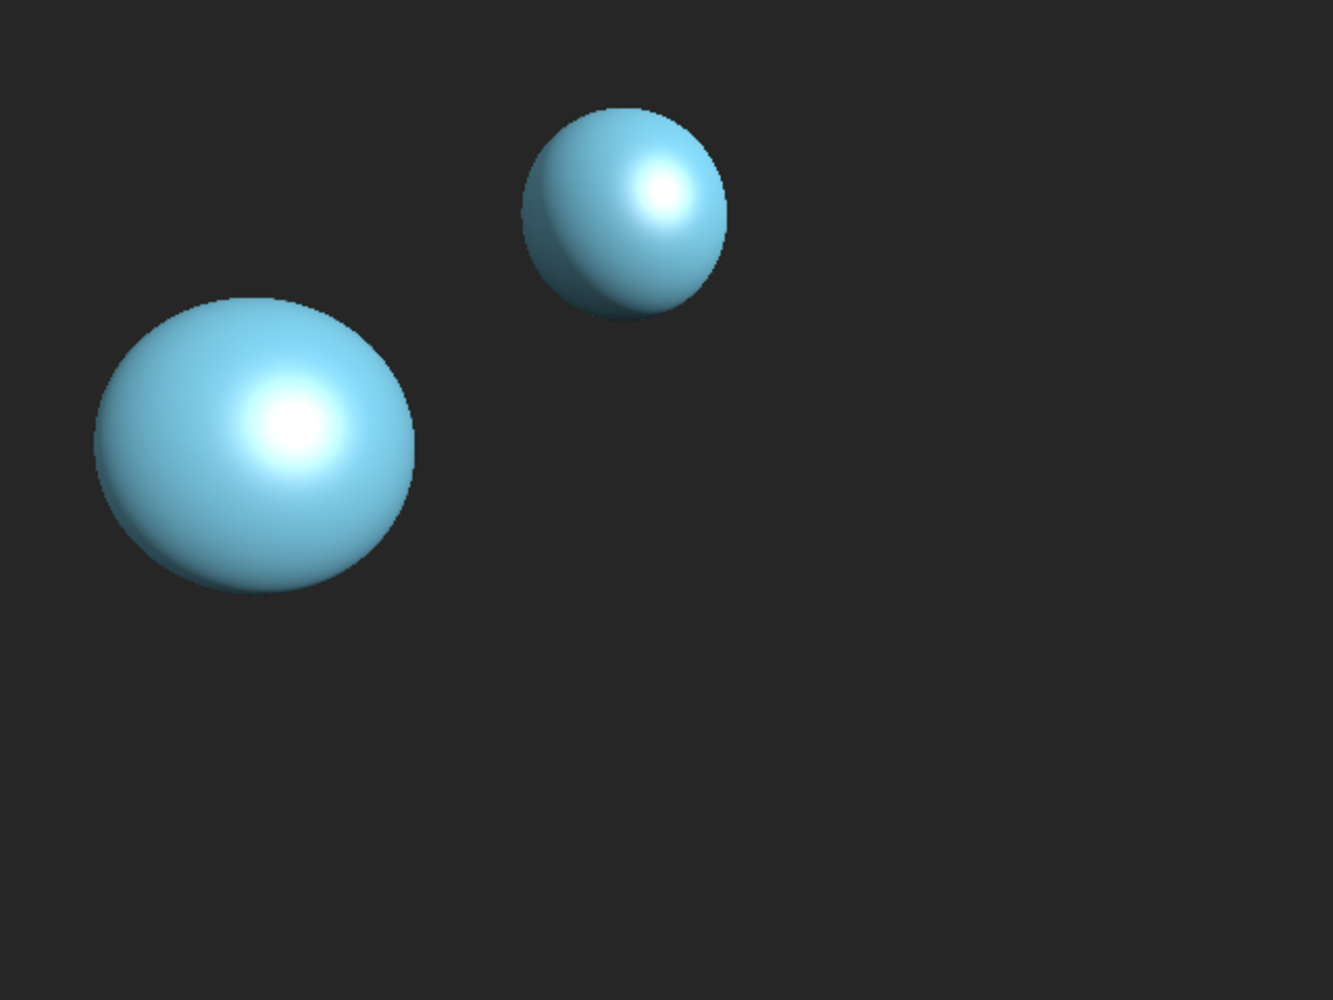
\includegraphics[width=0.3\textwidth]{img/sphere_tracing_distance_full.pdf}
            \newline
            Alle in der Szene definierten Objekte sind sichtbar. &
            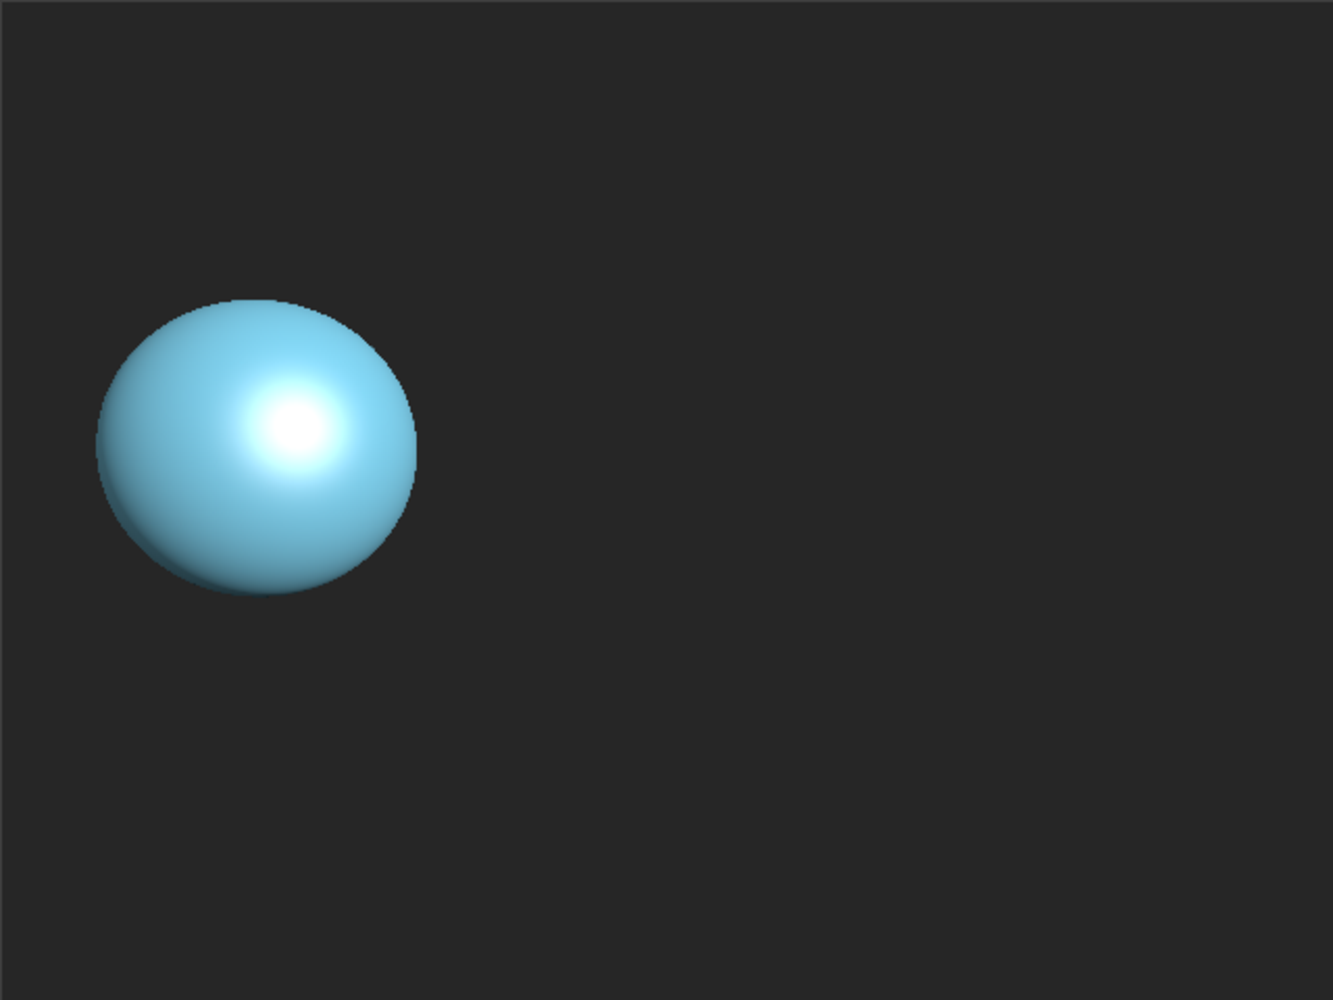
\includegraphics[width=0.3\textwidth]{img/sphere_tracing_distance_less.pdf} \newline
            Es ist nur noch das zum Betrachter näher liegende Objekt sichtbar. &
            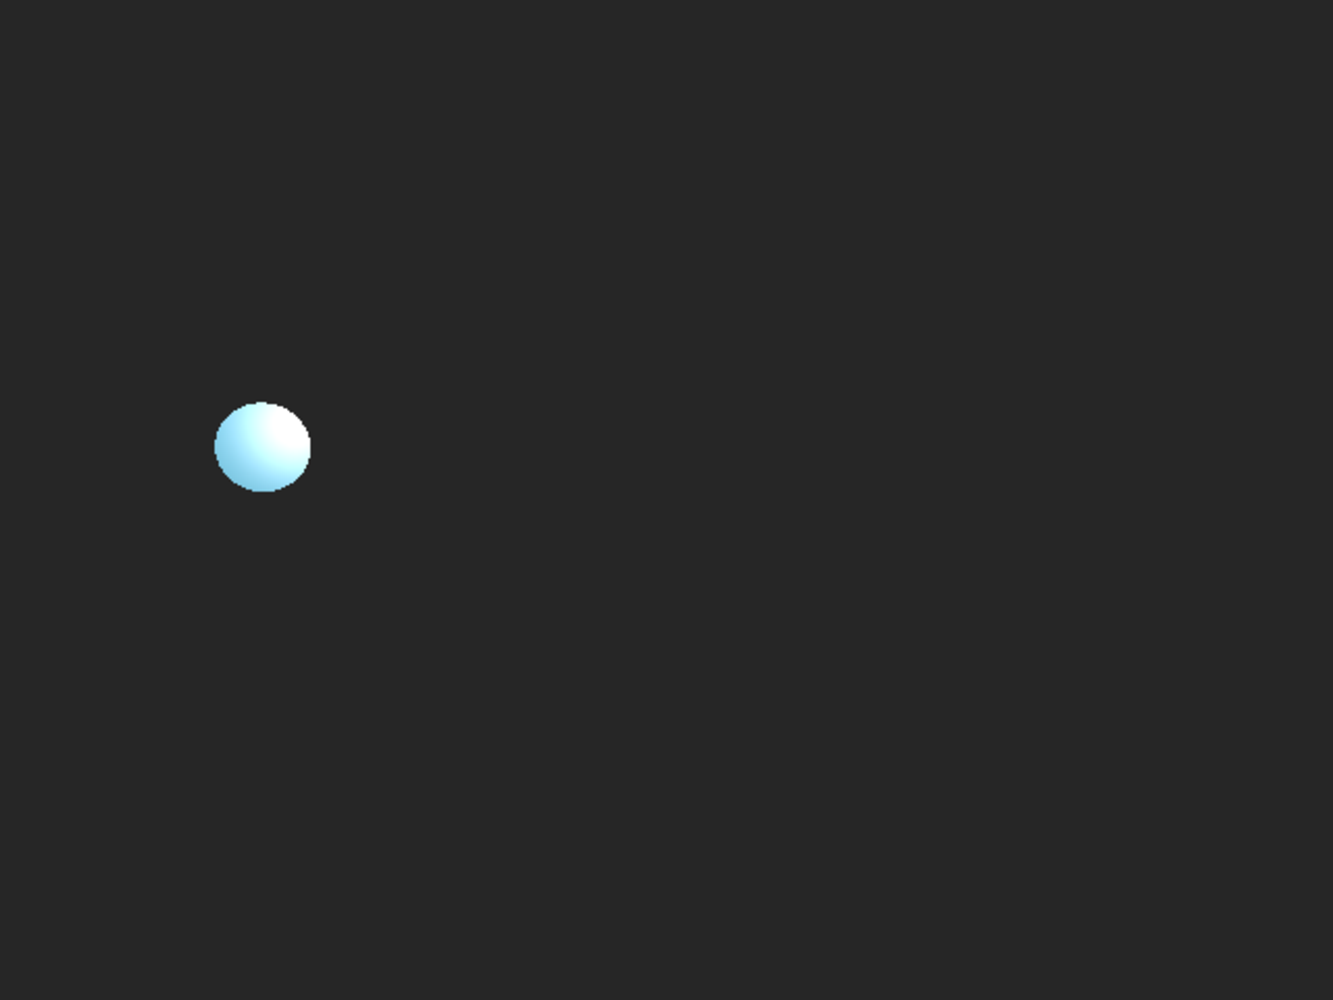
\includegraphics[width=0.3\textwidth]{img/sphere_tracing_distance_min.pdf} \newline
            Es ist nur noch das zum Betrachter näher liegende Objekt
            sichtbar, jedoch nicht mehr vollständig. \\
        \bottomrule
    \end{tabular}
\end{table}

\begin{table}[H]
    \centering
    \caption{Vergleich des Präzisions-Parameters anhand einer Beispielszene.}\label{table:sphere_tracing_precision}
    \begin{tabular}{p{0.3\textwidth}p{0.3\textwidth}p{0.3\textwidth}}
        \toprule
            \textbf{Präzision: \textit{0.00001}} &
            \textbf{Präzision: \textit{0.1}}     &
            \textbf{Präzision: \textit{1.0}}     \\
        \cmidrule(r){1-1}\cmidrule(lr){2-2}\cmidrule(l){3-3}
            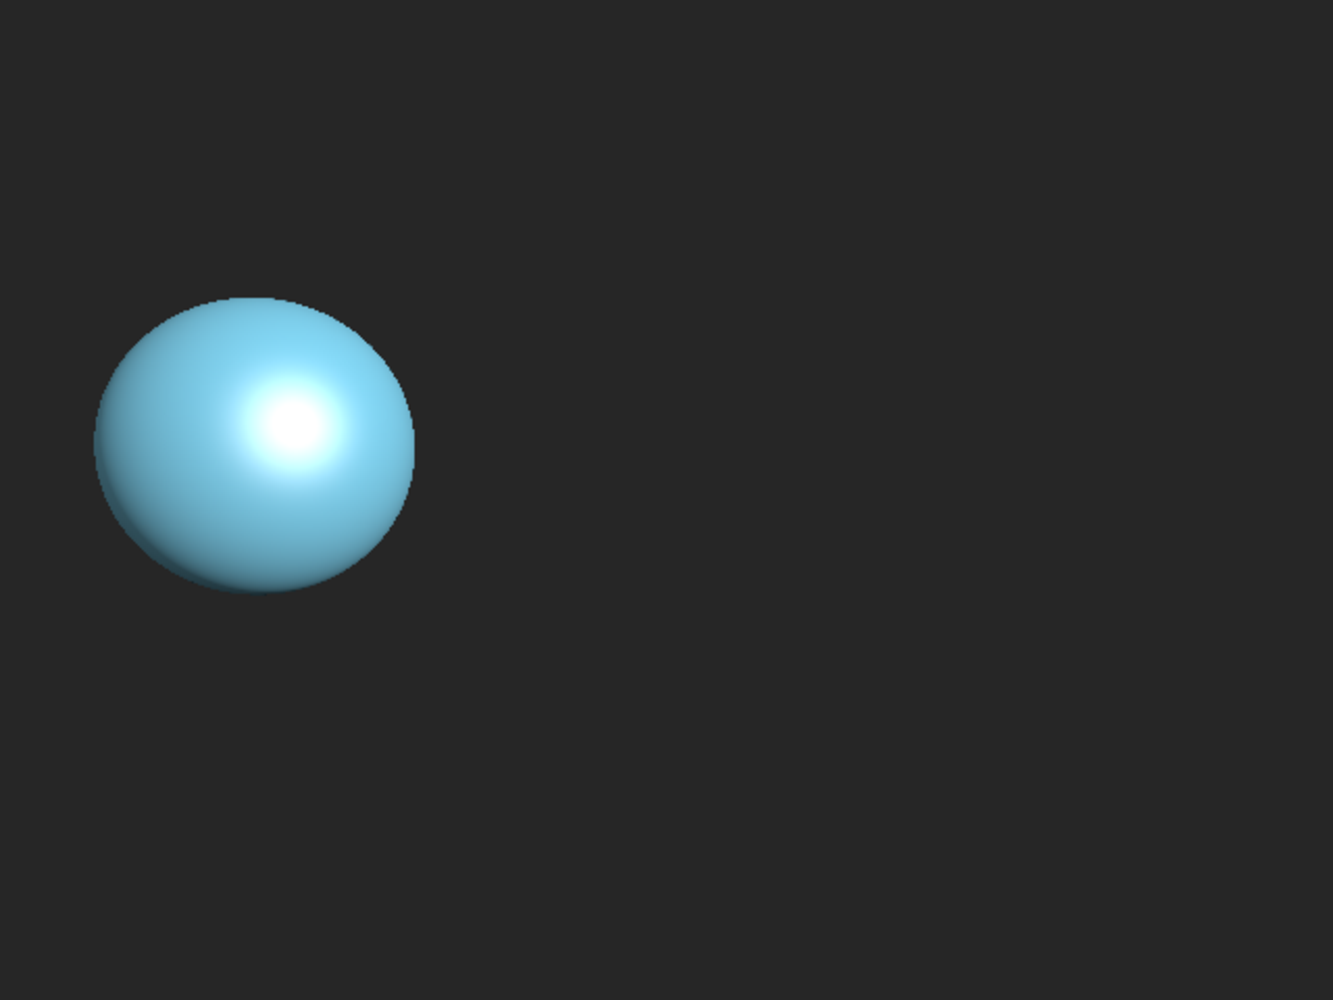
\includegraphics[width=0.3\textwidth]{img/sphere_tracing_precision_full.pdf} \newline
            Die Kugel ist weist keinerlei sichtbare Abstufungen auf. &
            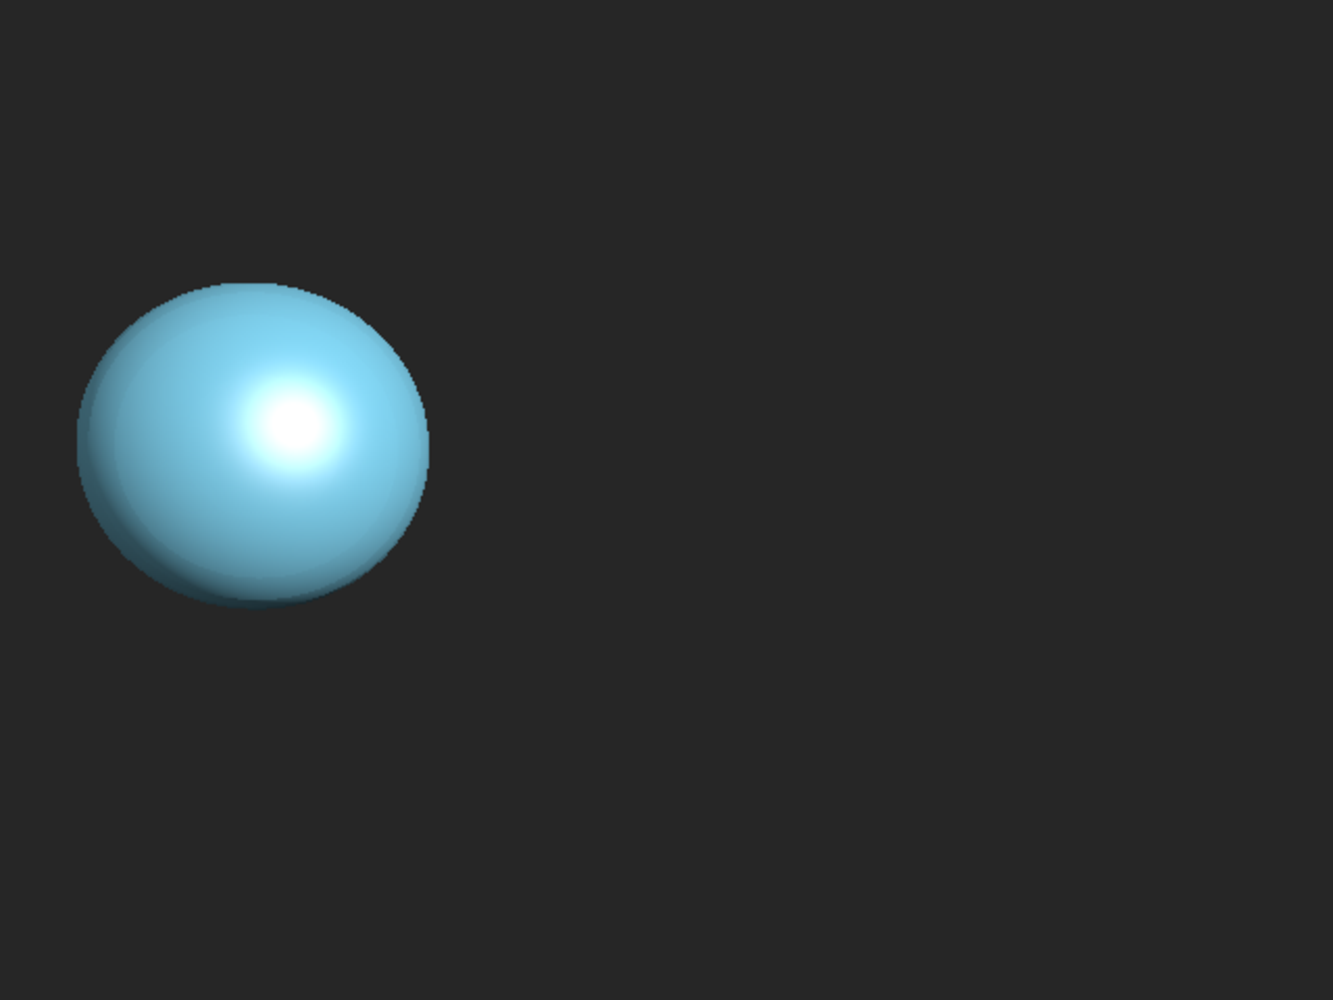
\includegraphics[width=0.3\textwidth]{img/sphere_tracing_precision_min.pdf} \newline
            Die Kugel weist am unteren linken Rand sichtbare Farbabstufungen auf. &
            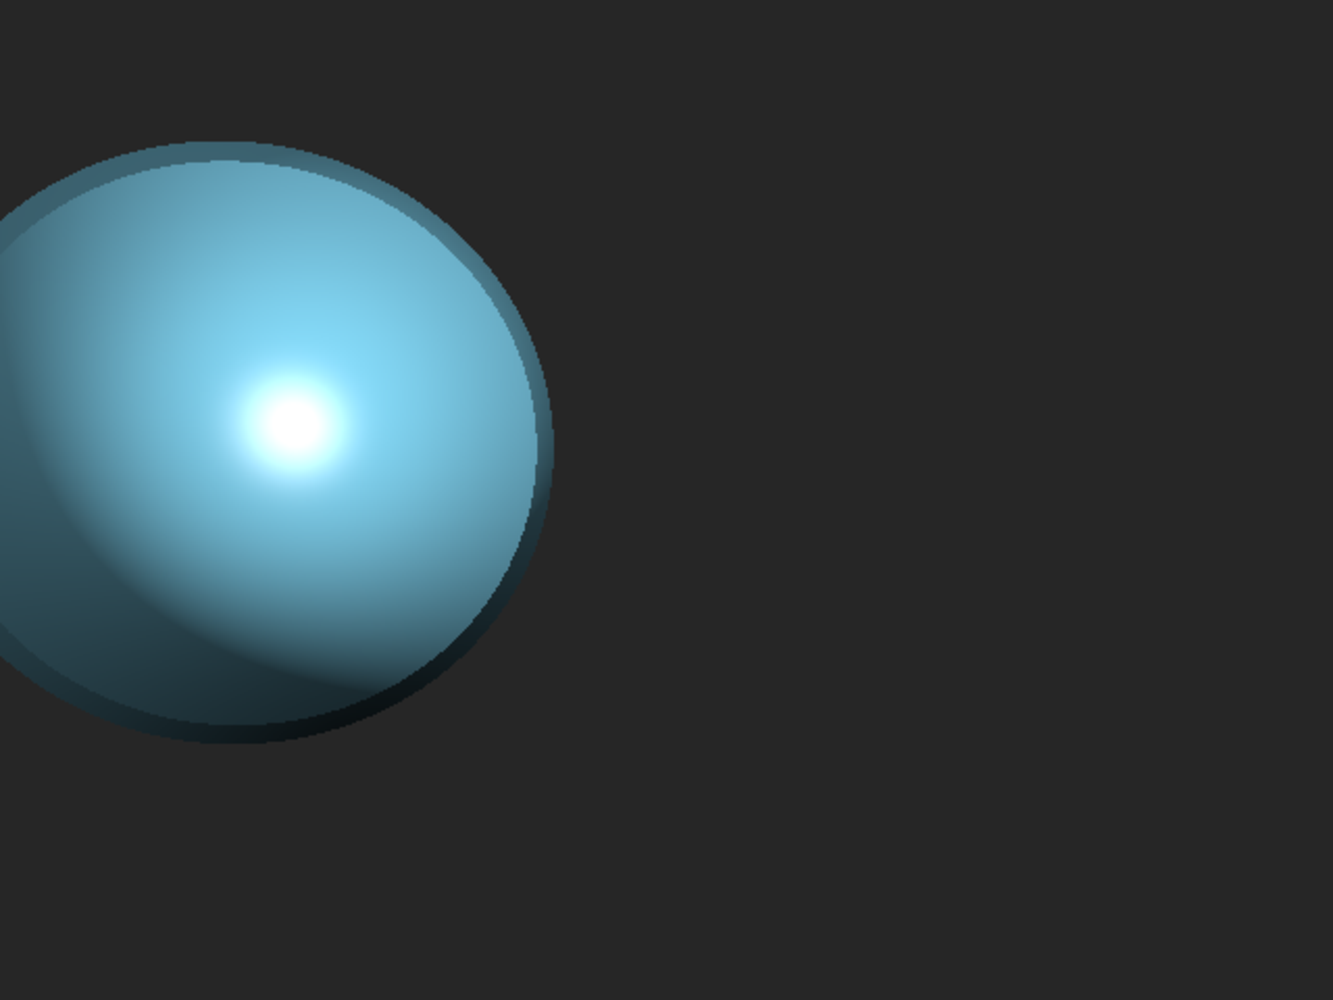
\includegraphics[width=0.3\textwidth]{img/sphere_tracing_precision_pos.pdf} \newline
            Die Kugel wird nicht mehr korrekt dargestellt. \\
        \bottomrule
    \end{tabular}
\end{table}

\begin{table}[H]
    \centering
    \caption{Vergleich des Parameters zur Bestimmung der Anzahl der
        Durchgänge anhand einer Beispielszene.}\label{table:sphere_tracing_steps}
    \begin{tabular}{p{0.3\textwidth}p{0.3\textwidth}p{0.3\textwidth}}
        \toprule
            \textbf{Anzahl Schritte: \textit{100}} &
            \textbf{Anzahl Schritte: \textit{10}}  &
            \textbf{Anzahl Schritte: \textit{5}}   \\
        \cmidrule(r){1-1}\cmidrule(lr){2-2}\cmidrule(l){3-3}
            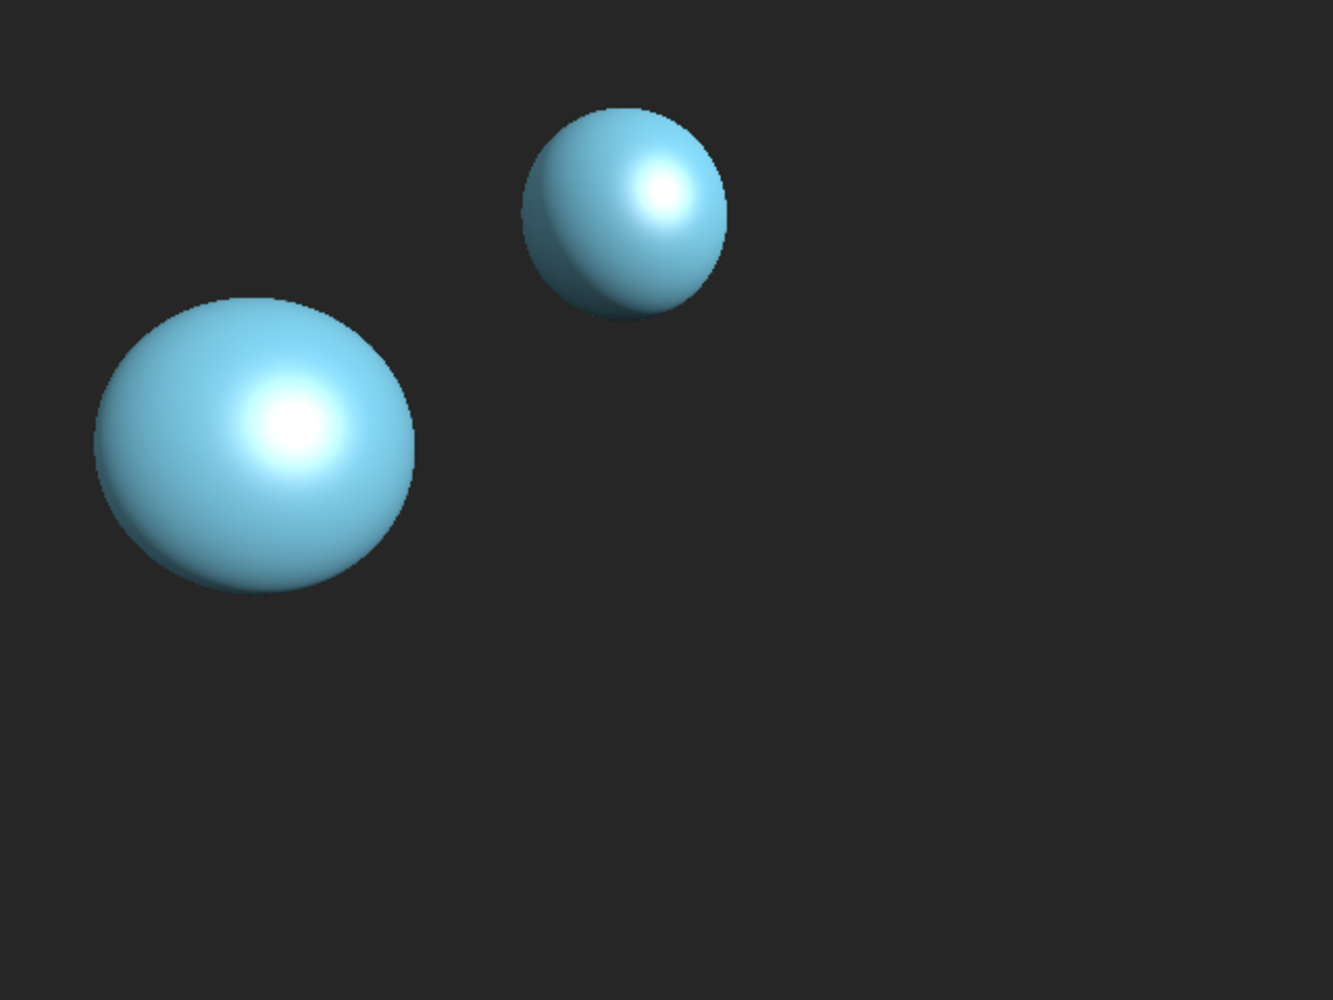
\includegraphics[width=0.3\textwidth]{img/sphere_tracing_steps_full.pdf} \newline
            Alle in der Szene definierten Objekte sind korrekt sichtbar. &
            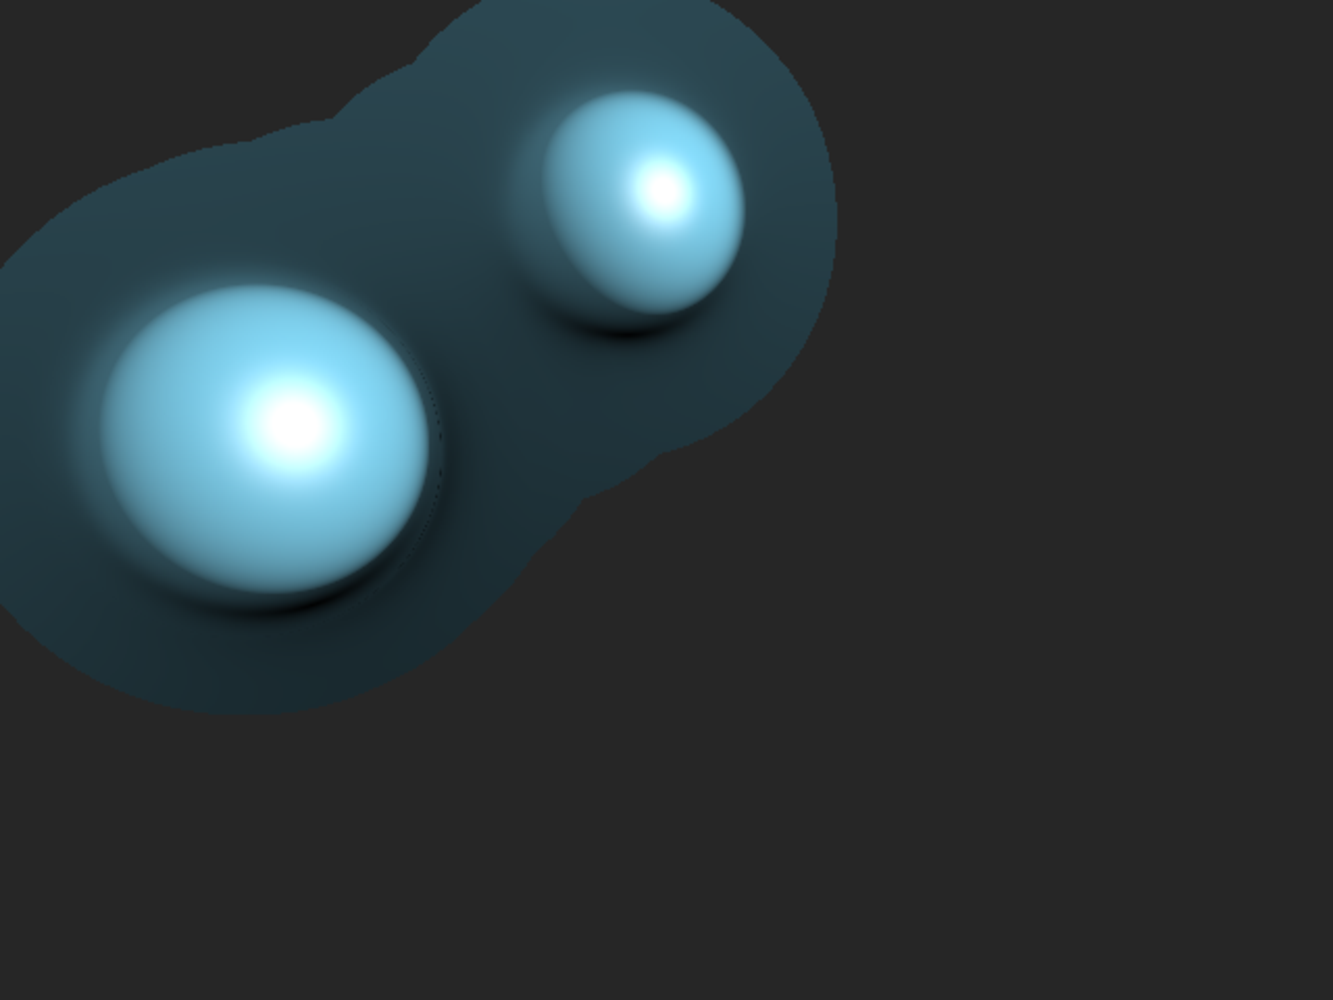
\includegraphics[width=0.3\textwidth]{img/sphere_tracing_steps_less.pdf} \newline
            Die Grenze zwischen den in der Szene definierten Objekten
            ist bereits nicht mehr eindeutig. &
            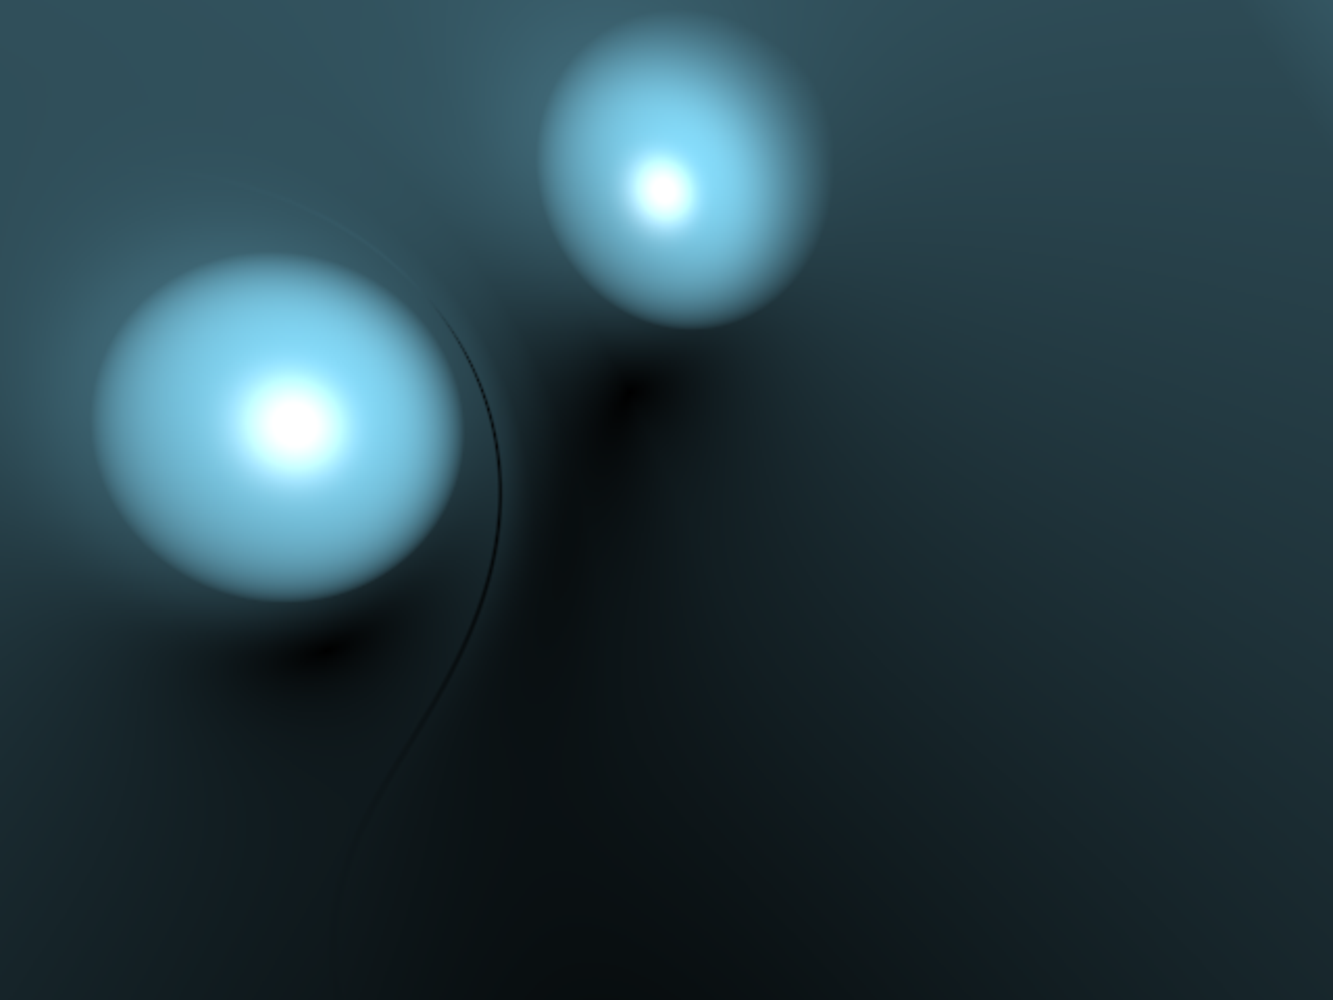
\includegraphics[width=0.3\textwidth]{img/sphere_tracing_steps_min.pdf} \newline
            Die Szene ist als solche nicht mehr erkennbar, es erfolgt
            keine klare Trennung zwischen den einzelnen Objekten mehr.  \\
        \bottomrule
    \end{tabular}
\end{table}

Von den unter~\autoref{subsec:implicit_surfaces_ops} beschriebenen
Operationen wurden die Operationen \textit{Vereinigung}, \textit{Subtraktion} sowie
\textit{Intersektion} umgesetzt.

\begin{lstlisting}[language=GLSL,caption={Umsetzung der Operationen
        \textit{Vereinigung}, \textit{Subtraktion} sowie
        \textit{Intersektion} für implizite Oberflächen in
        GLSL.},label={alg:glsl_ops},captionpos=b,emph={subtract,merge,intersect}]
// Returns the signed distance for a substraction of given signed
// distance a to signed distance b.
float subtract(float a, float b)
{
    return max(-b, a);
}

// Returns the signed distance for a merge of given signed
// distance a and signed distance b.
vec2 merge(vec2 a, vec2 b)
{
    return min(a, b);
}

// Returns the signed distance for a intersection  of given signed
// distance a and signed distance b.
float intersect(float a, float b)
{
    return (a > b) ? a : b;
}
\end{lstlisting}

Von den unter~\autoref{subsec:implicit_surfaces_primitives} beschriebenen
Primitiven wurden die Primitiven \textit{Ebene} sowie \textit{Kugel} umgesetzt.

\begin{lstlisting}[language=GLSL,caption={Umsetzung der Primitiven
        \textit{Ebene} und \textit{Kugel} in Form von impliziten
        Oberflächen in
        GLSL.},label={alg:glsl_primitives},captionpos=b,emph={plane,sphere,box}]
// Returns the signed distance to a plane for the given position.
float plane(vec3 position)
{
    return position.y;
}

// Returns the signed distance to a sphere with given radius for the
// given position.
float sphere(vec3 position, float radius)
{
    return length(position) - radius;
}

// Returns the signed distance to a box with given dimension for the
// given position.
float box(vec3 position, vec3 dimension)
{
    position = abs(position) - dimension;
    return max(max(position.x, position.y), position.z);
}
\end{lstlisting}

Verwendete Parameter sind dabei jeweils die (gewünschte) Position des Objektes
(\textit{vec3 position}) sowie der Radius bzw.\ die Dimension
(\textit{float radius} bzw. \textit{vec3 dimension}).

Als Beleuchtungsmodell wurde das
unter~\autoref{sec:rendering_implicit_surfaces} beschriebene
Phong-Beleuchtungsmodell umgesetzt.

\begin{lstlisting}[language=GLSL,caption={Umsetzung des
        Phong-Beleuchtungsmodelles in
        GLSL.},label={alg:glsl_lighting},captionpos=b,emph={calcLighting}]
// Calculates the lighting for the given position, normal and direction,
// the given light (position and color) respecting the 'material'.
//
// This is mainly applying the phong lighting model inlcuding shadows.
//
// Returns the calculated color as three-dimensional vector.
vec3 calcLighting(vec3 normal, vec3 rayDirection) {

    vec3 lightDirection     = normalize(vec3(0.0, 4.0, 5.0));

     float kDirectLight      = 0.1;
     float shadows           = calcShadows(position, lightDirection);
     vec3  direct            = vec3(kDirectLight * shadows);

    vec3 ambientColor       = vec3(0.05, 0.15, 0.2);
    float kAmbient          = clamp(0.5 + 0.5 * normal.y, 0.0, 1.0);
    vec3 ambient            = kAmbient * ambientColor;

    vec3 diffuseColor       = vec3(0.2, 0.6, 0.8);
    float kDiffuse          = clamp(dot(lightDirection, normal), 0.0, 1.0);
    vec3 diffuse            = kDiffuse * diffuseColor;

    vec3 specularColor      = vec3(1.0);
    float kSpecularExponent = 24.0;
    vec3 h                  = normalize(-rayDirection + lightDirection);
    float nFacing           = clamp(dot(lightDirection, normal), 0.0, 1.0);
    float kSpecular         = pow(clamp(dot(h, normal), 0.0, 1.0), kSpecularExponent);
    vec3 specular           = nFacing * kSpecular * specularColor;

     vec3 light              = ambient + diffuse + specular + direct;
     vec3 color              = material * light;
 
     return color;
}
\end{lstlisting}

Als Parameter werden hier ein Normalvektor einer Oberfläche ($\bm{n}$)
sowie die Richtung eines eingehenden Strahles (also die Blichrichtung
des Betrachters bzw.\ der Kamera, $\vv{V}$) benötigt.
Wie oben ersichtlich ist, wird zuerst die Richtung der Lichtquelle definiert,
danach werden die einzelnen Anteile des Lichtes $I_{\text{ambient}}$,
$I_{\text{diffuse}}$ sowie $I_{\text{sepcular}}$ berechnet.

Die Normale einer Oberfläche wird wie
unter~\autoref{sec:rendering_implicit_surfaces_lighting} beschrieben
berechnet.

\begin{lstlisting}[language=GLSL,caption={Berechnung der Normalen einer
        impliziten Oberfläche in
        GLSL.},label={alg:glsl_normal},captionpos=b,emph={calcNormal}]
// Calculates the normal vector for given position with respect to a
// certain offset given by epsilon.
vec3 calcNormal(in vec3 position, in float epsilon) {

    vec3 eps = vec3(epsilon, 0.0, 0.0);
    vec3 normal  = vec3(
        scene(position + eps.xyy).x - scene(position - eps.xyy).x,
        scene(position + eps.yxy).x - scene(position - eps.yxy).x,
        scene(position + eps.yyx).x - scene(position - eps.yyx).x
    );

    return normalize(normal);
}
}
\end{lstlisting}

Verwendete Parameter sind dabei ein Punkt der Oberfläche eines Objektes
(\textit{vec3 position}) sowie die minimale Inkrementation eines
(Licht-) Strahles ($\varepsilon$). Wie zuvor erwähnt, sollte
für $\varepsilon$ ein möglichst kleiner Wert gewählt werden, daher wird
standardmässig der Wert \textit{0.1} verwendet.

Bei der Funktion \textit{scene} handelt es sich um eine Distanzfunktion
$f$ gemäss~\autoref{ssubsec:distance_functions}. Diese definiert
schliesslich, was an einem gegebenen Punkt dargestellt wird.

\begin{lstlisting}[language=GLSL,caption={Distanzfunktion $f$ in
        GLSL.},label={alg:glsl_distance_func},captionpos=b,emph={scene}]
// Defines the scene which will be drawn at given position.
float scene(in vec3 position) {
{
    float sphereRadius = 1.0;
    vec3  sphereOffset = vec3(-2.0, 1.0, -2.0);

    float res = sphere(position - sphereOffset, sphereRadius);

    return res;
}
\end{lstlisting}

In diesem Beispiel wird eine Kugel mit Radius \textit{1.0} dargestellt.
Diese wird auf der \textit{X}-Achse um -2 Einheiten, auf der
\textit{Y}-Achse um 1 Einheit und auf der \textit{Z}-Achse um -2
Einheiten verschoben (Translation).

Wie in~\autoref{sec:rendering_implicit_surfaces_shadows} beschrieben,
wurden weiche Schatten implementiert.

\begin{lstlisting}[language=GLSL,caption={Funktion zur Berechnung von
        weichen Schatten  in
        GLSL.},label={alg:glsl_soft_shadows},captionpos=b,emph={calcShadows}]
// Calcuates soft shadows for the given ray origin and direction.
//
// Returns a shadow color for the given origin between 0.0 and 1.0.
float calcShadows(in vec3 rayOrigin, in vec3 rayDirection)
{
    float shadow            = 1.0;
    float minimalDistance   = 0.01;
    float maximalDistance   = 2.5;
    float convergePrecision = 0.000001;
    float kShadow           = 8.0;
    float currentDistance   = minimalDistance;

    while (currentDistance < maximalDistance) {
        vec3 ray = rayOrigin + rayDirection * currentDistance;
        float estimatedDistance = scene(ray);

        if (estimatedDistance < convergePrecision) {
            return 0.0;
        }

        float penumbraFactor = estimatedDistance / currentDistance;
        shadow = min(shadow, kShadow * penumbraFactor);
        currentDistance += estimatedDistance;
    }

    return clamp(shadow, 0.0, 1.0);

}
\end{lstlisting}

Verwendete Parameter sind dabei der Ursprung eines Strahles
(\textit{vec3 rayOrigin}), sowie die Richtung eines Strahles
(\textit{vec3 rayDirection}). 

\begin{table}[H]
    \centering
    \caption{Vergleich des Skalierungsfaktors \textit{kShadow} für
        weiche Schatten anhand einer
        Beispielszene.}\label{table:sphere_tracing_shadows}
    \begin{tabular}{p{0.3\textwidth}p{0.3\textwidth}p{0.3\textwidth}}
        \toprule
            \textbf{kShadow: \textit{8.0}} &
            \textbf{kShadow: \textit{16.0}}   &
            \textbf{kShadow: \textit{32.0}}   \\
        \cmidrule(r){1-1}\cmidrule(lr){2-2}\cmidrule(l){3-3}
            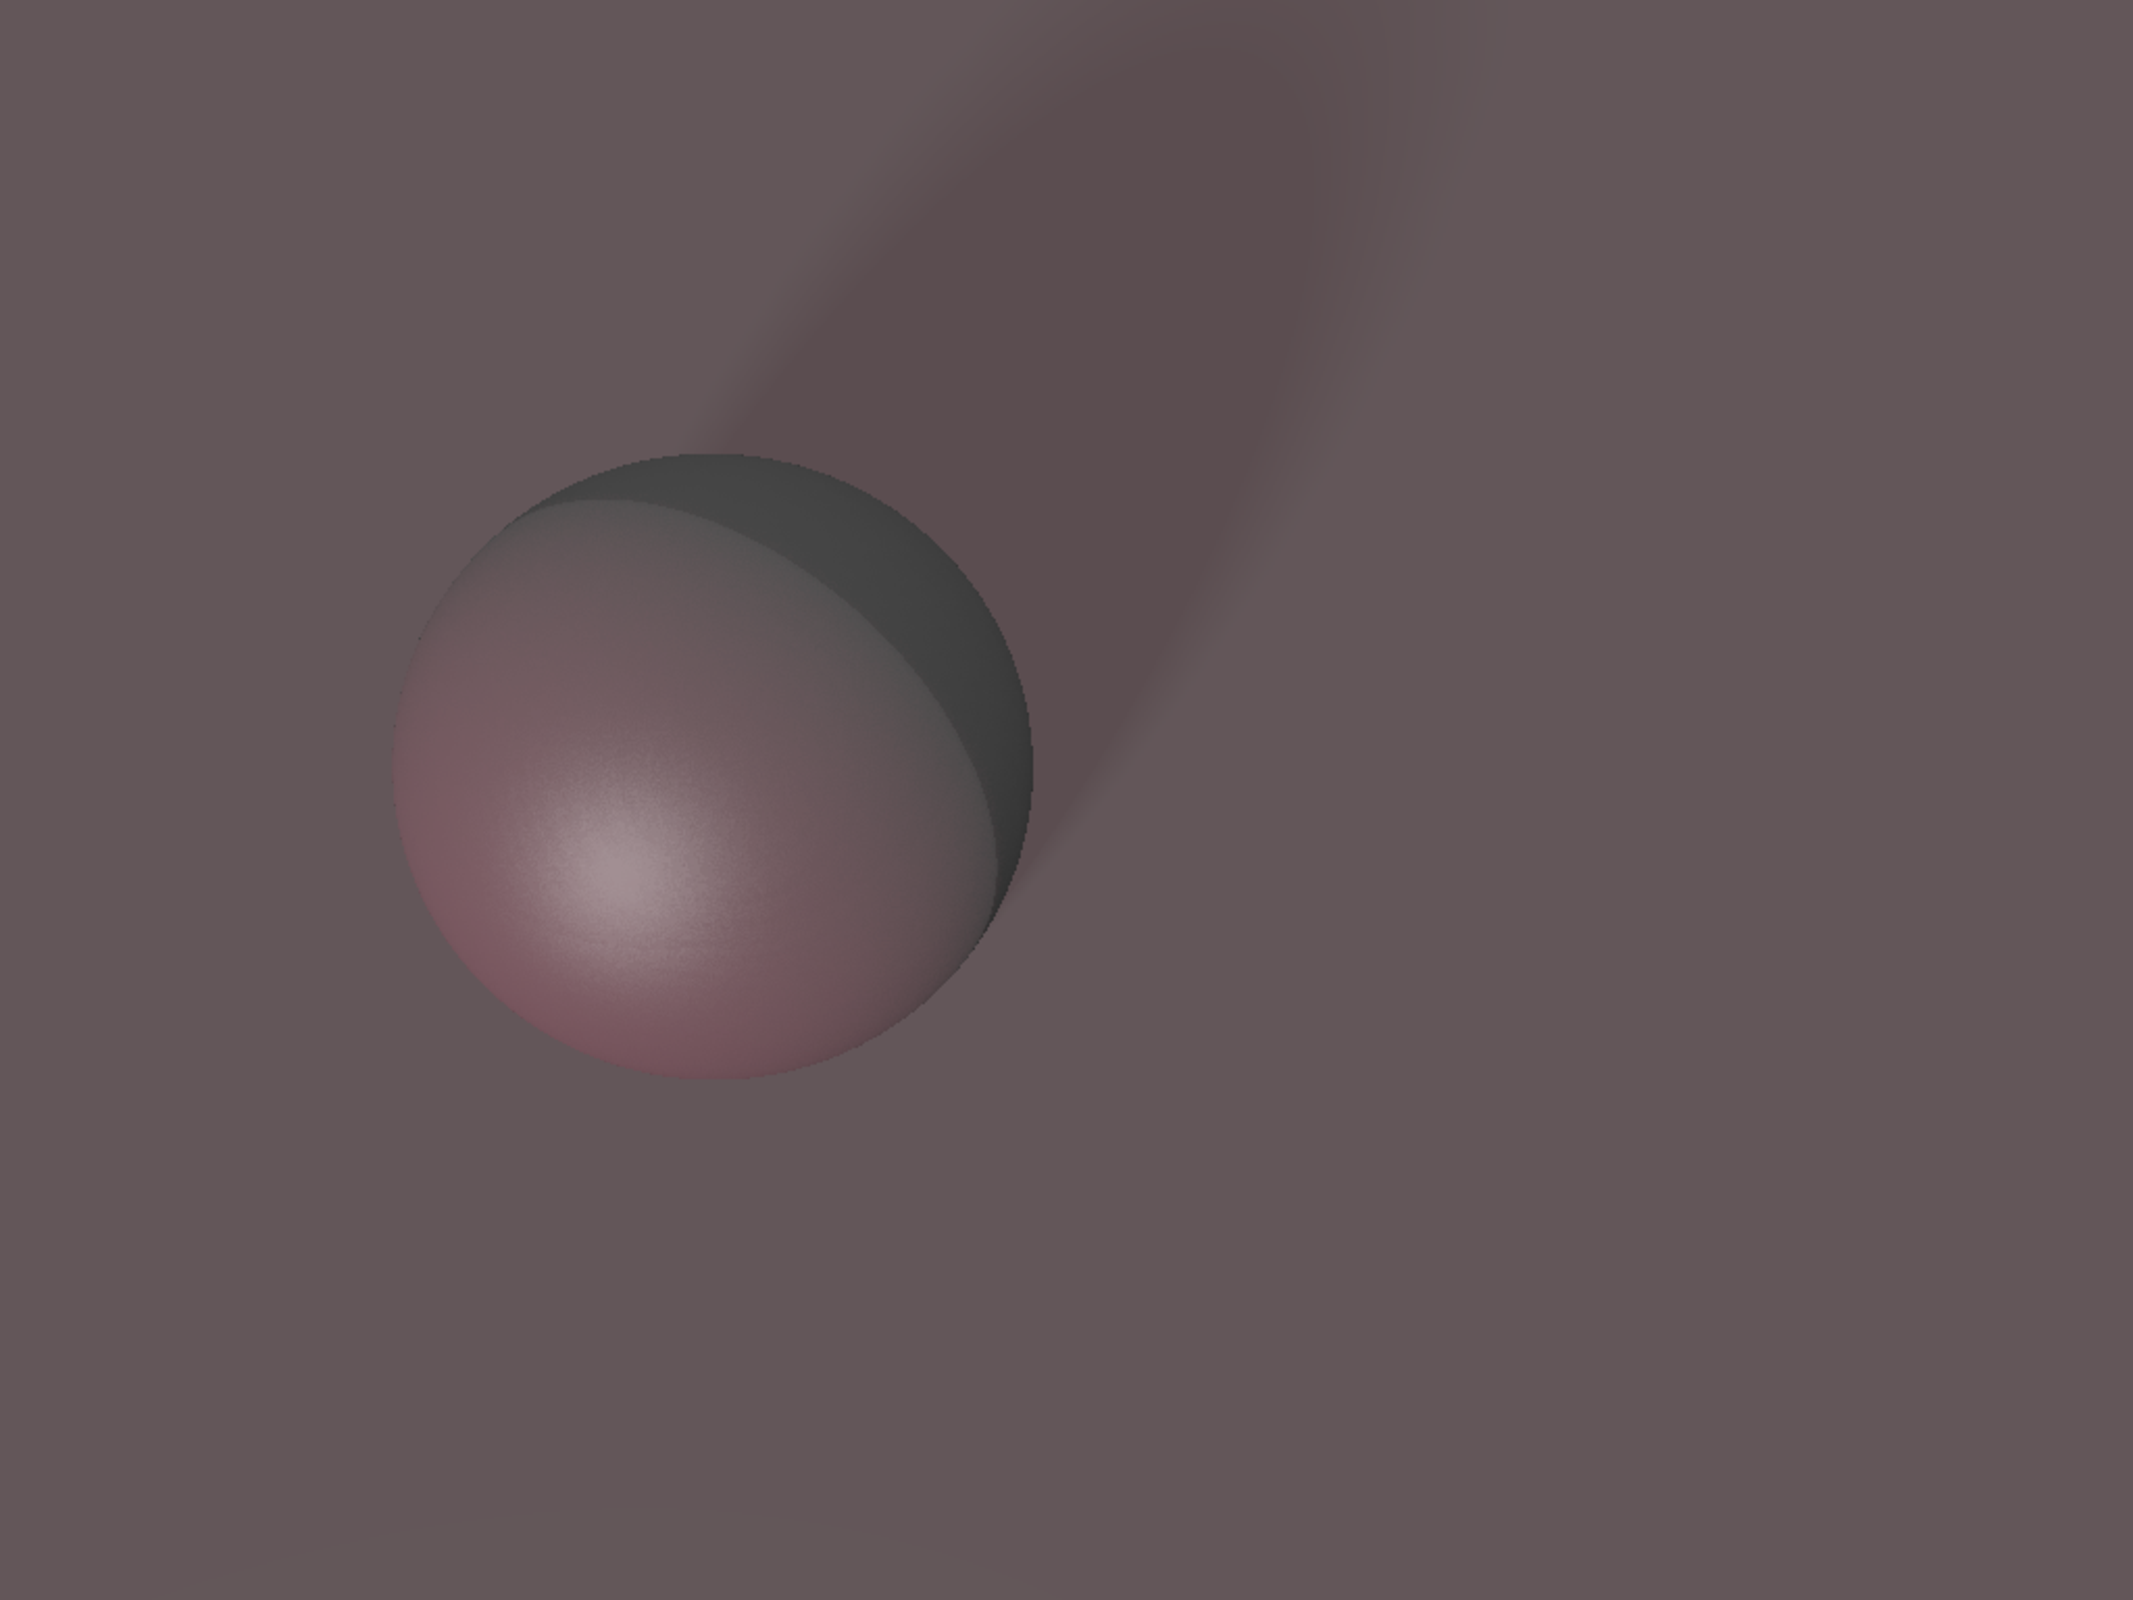
\includegraphics[width=0.3\textwidth]{img/sphere_tracing_shadows_8.pdf} \newline &
            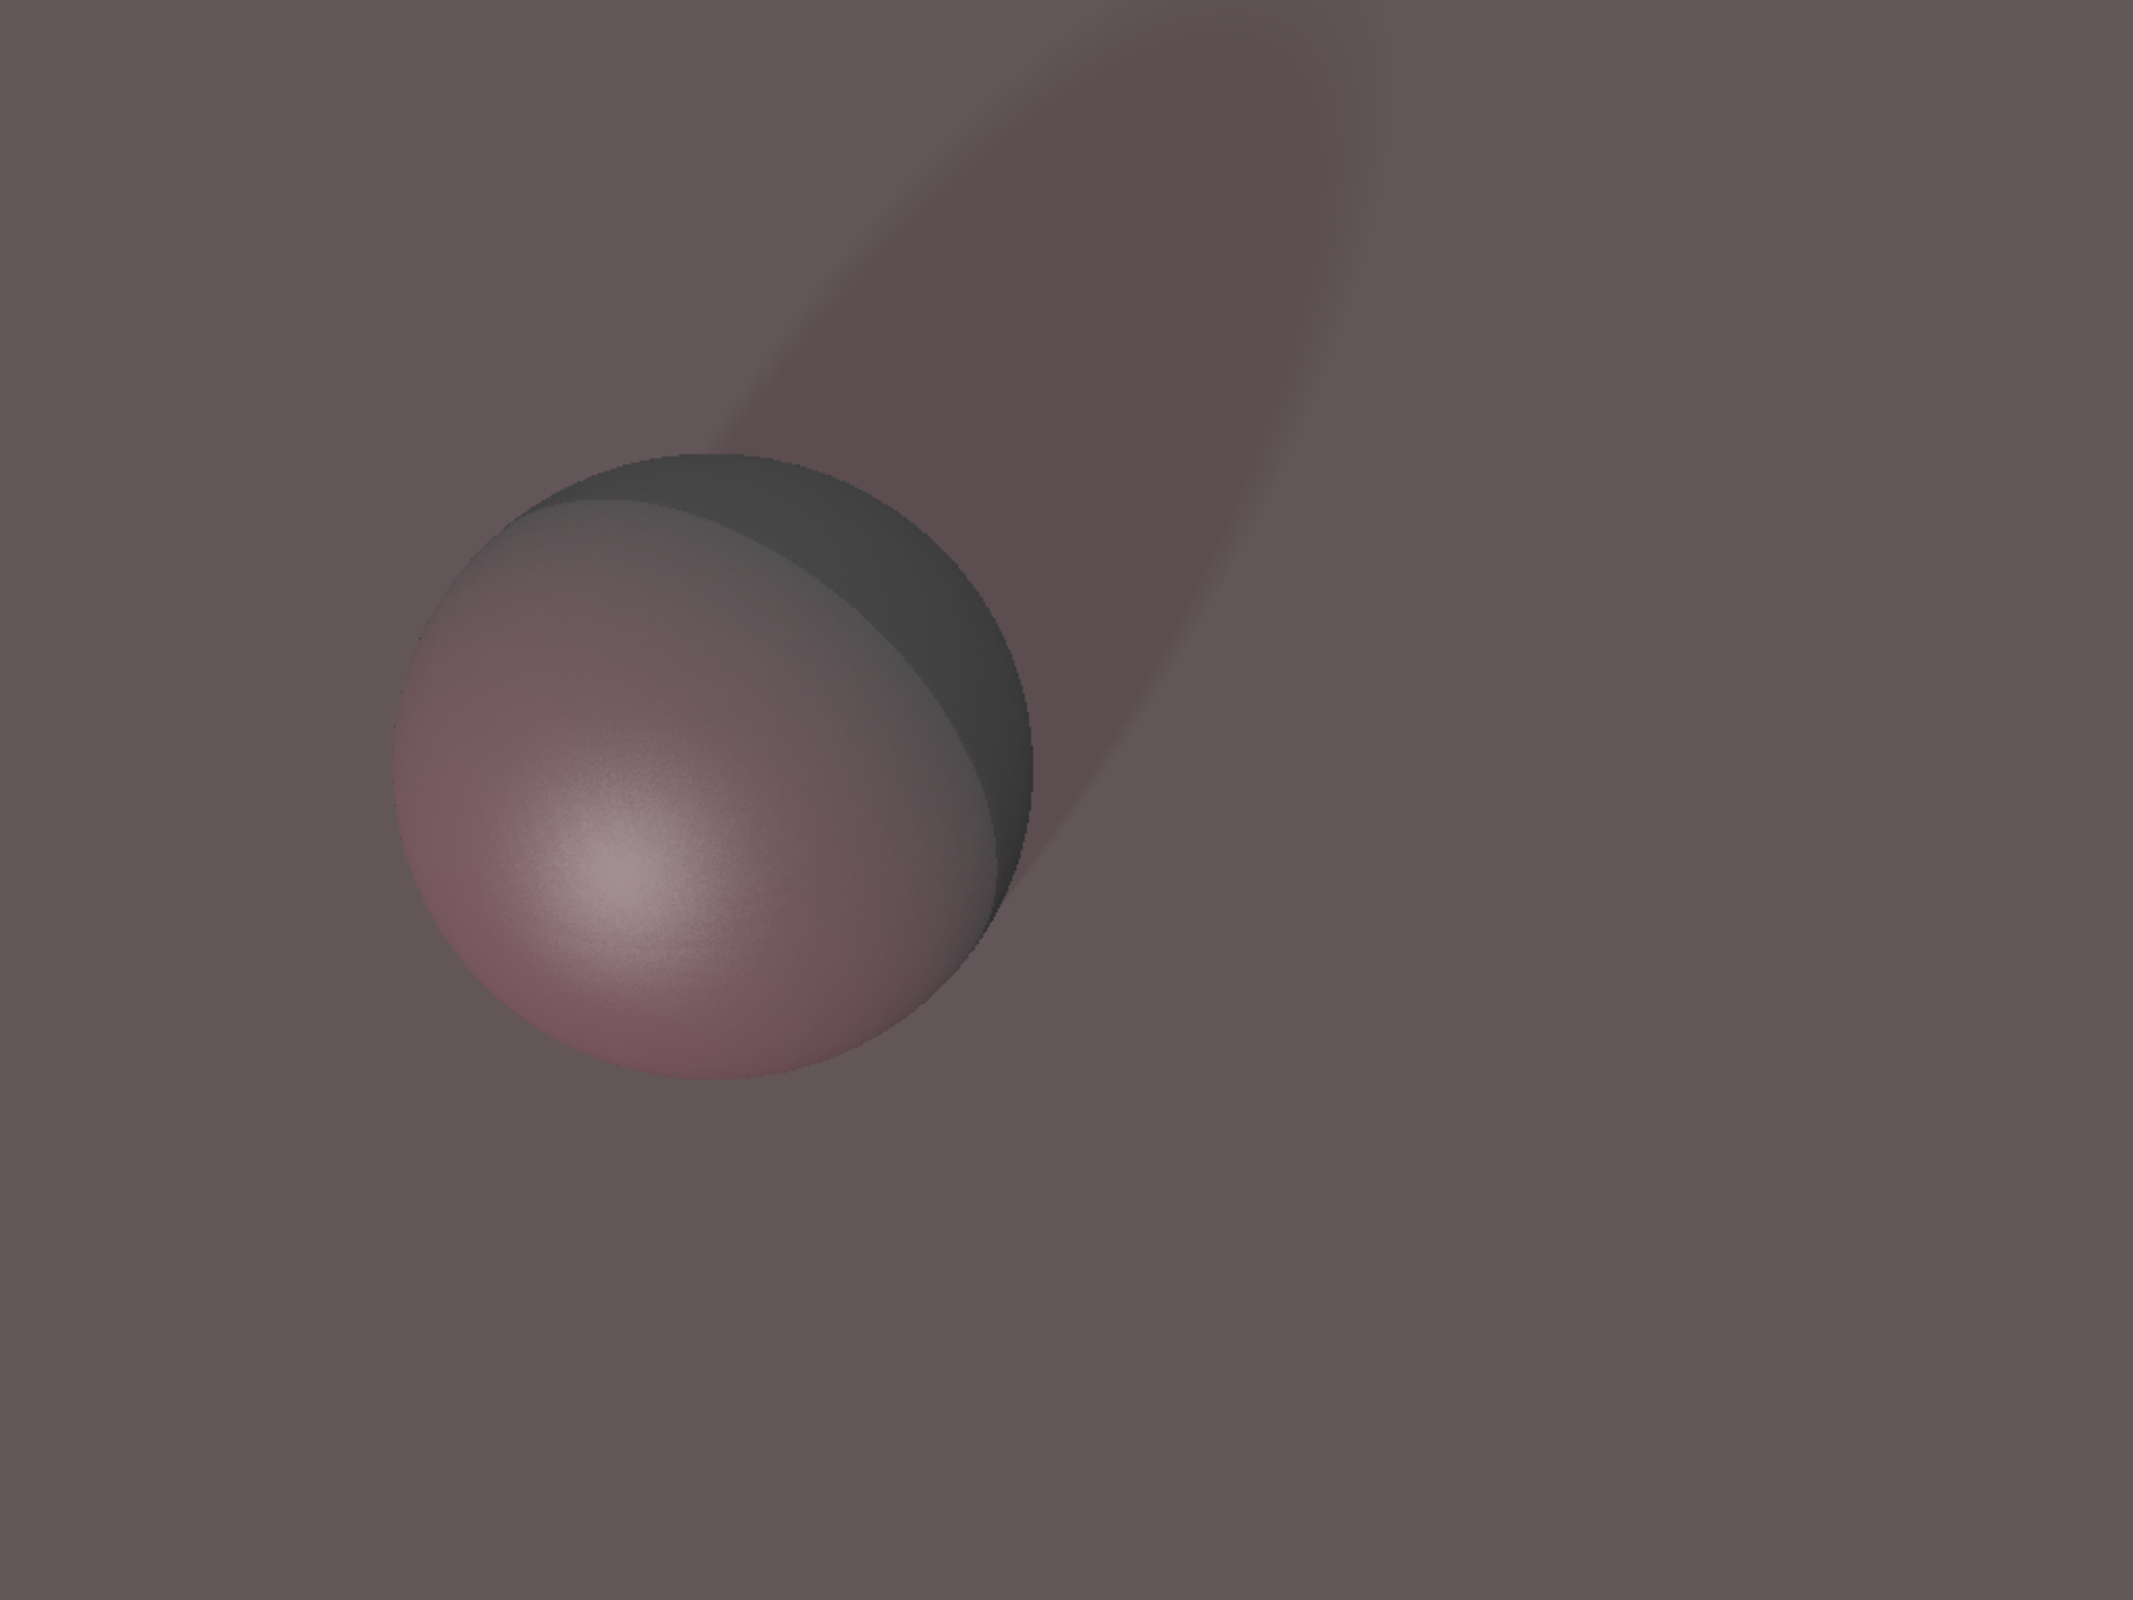
\includegraphics[width=0.3\textwidth]{img/sphere_tracing_shadows_16.pdf} \newline &
            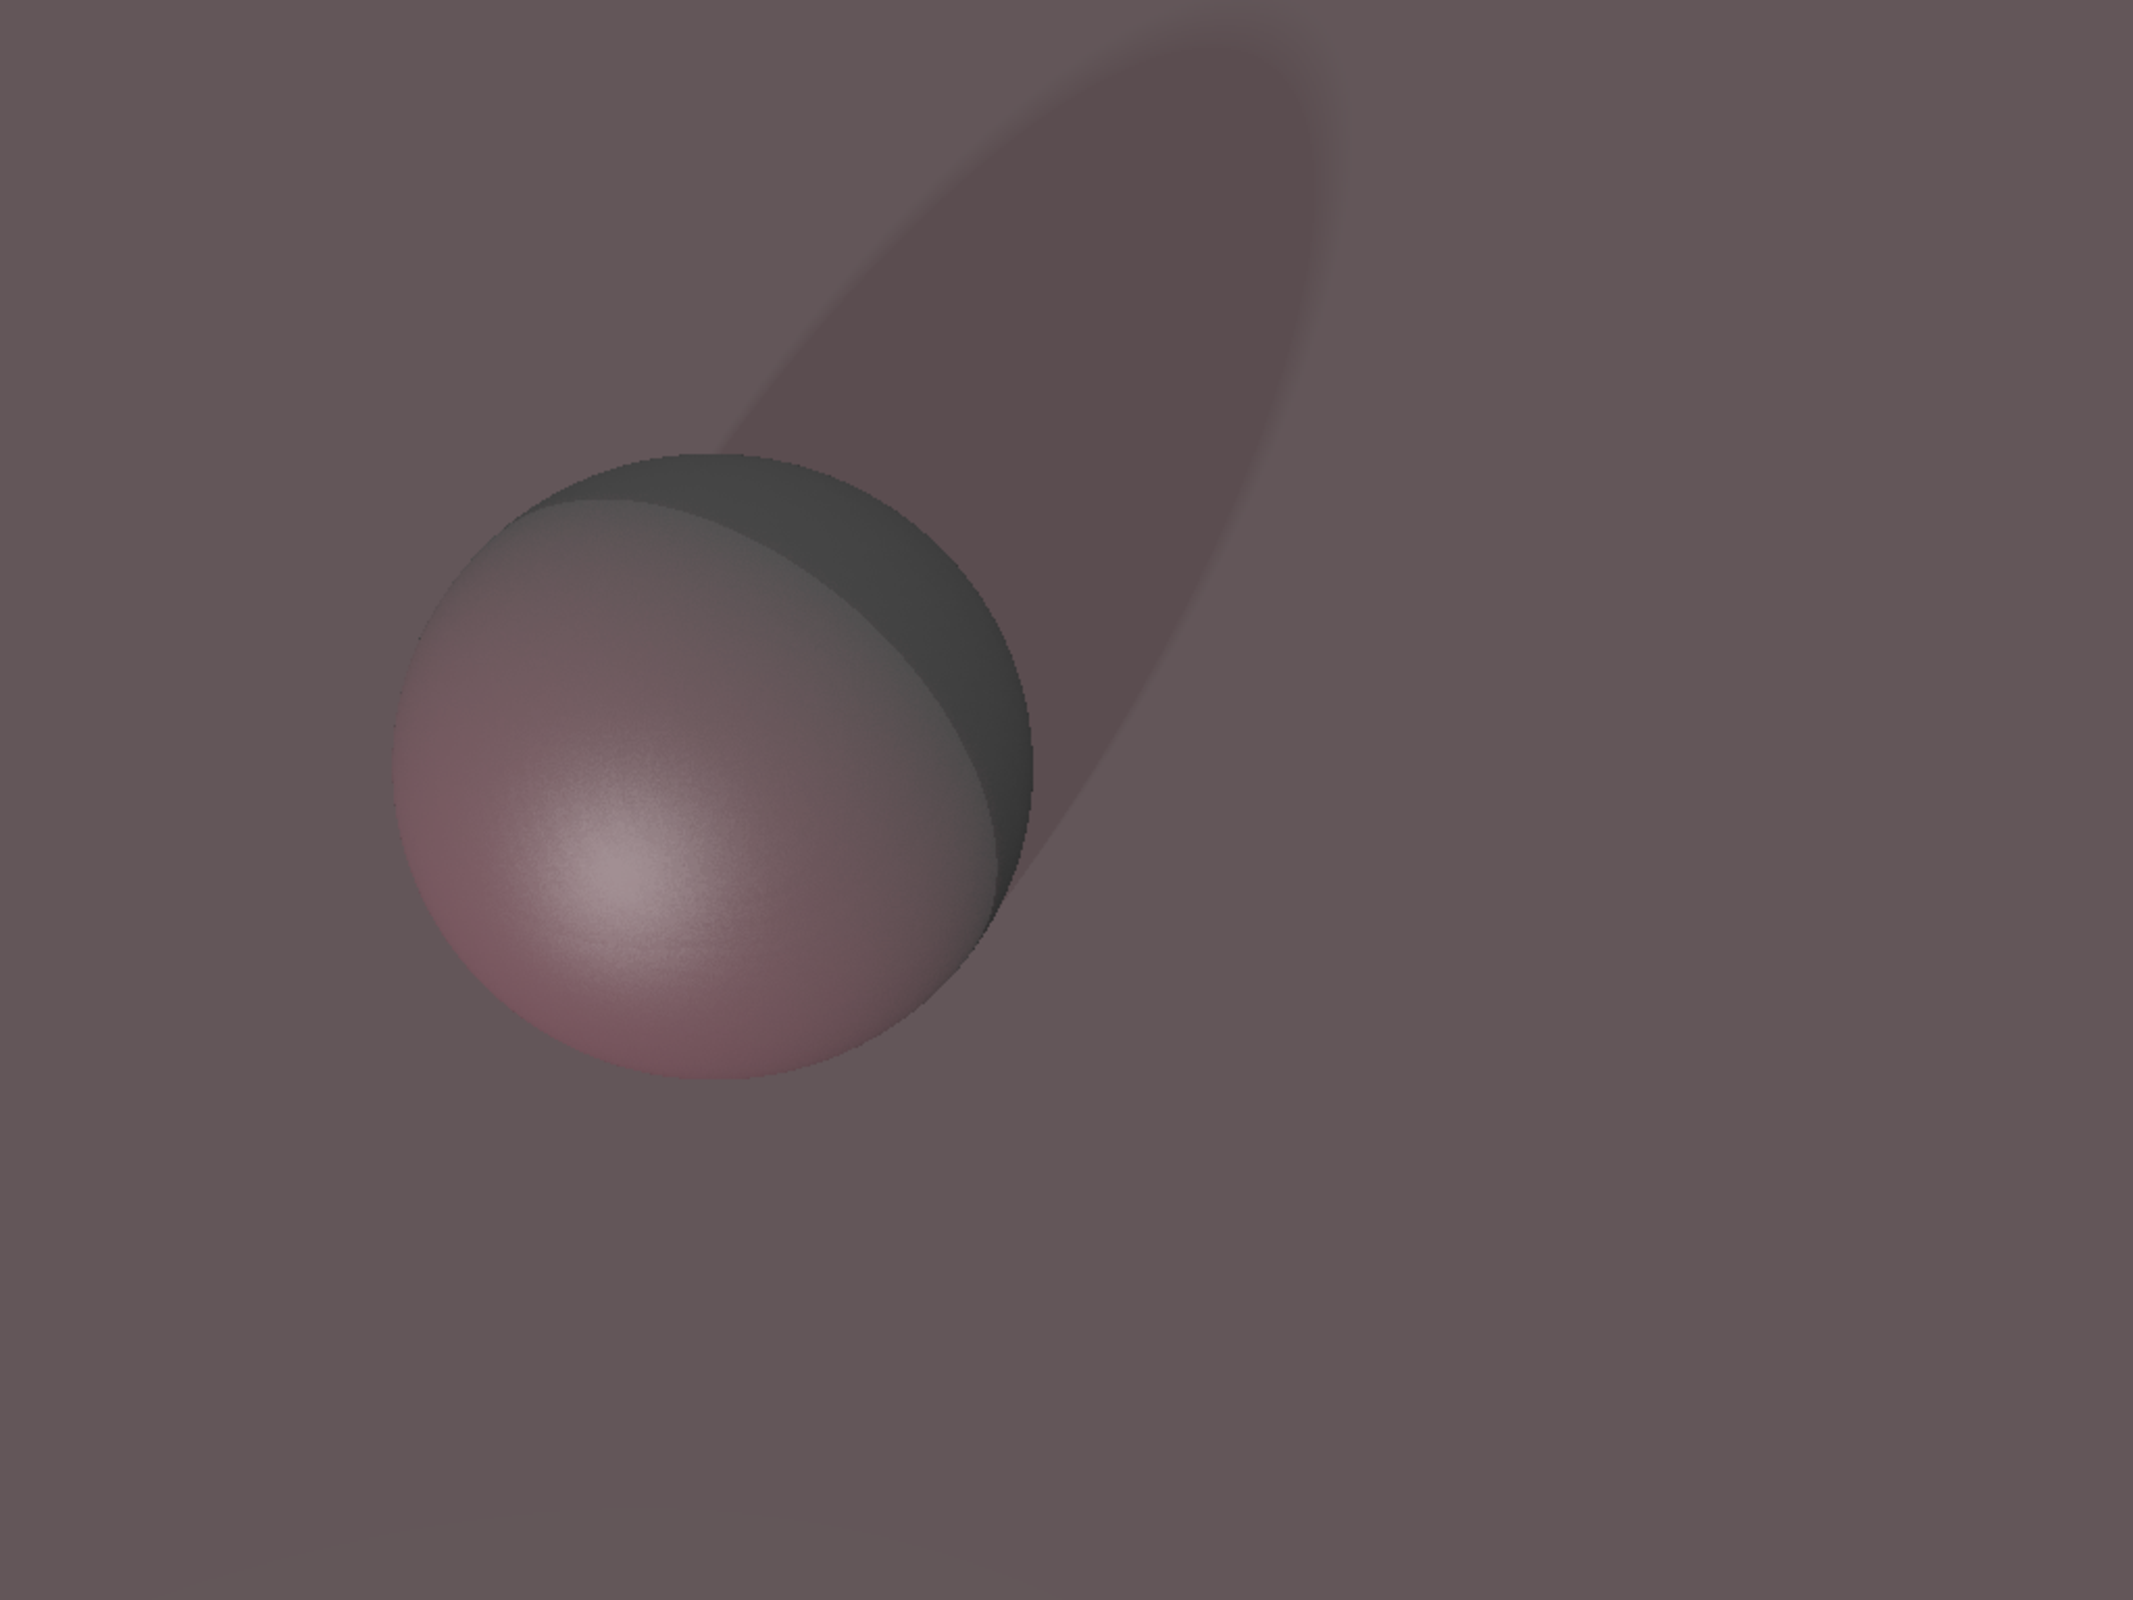
\includegraphics[width=0.3\textwidth]{img/sphere_tracing_shadows_32.pdf} \newline \\
        \bottomrule
    \end{tabular}
    \begin{tabular}{p{0.3\textwidth}p{0.3\textwidth}p{0.3\textwidth}}
        \toprule
            \textbf{kShadow: \textit{64.0}} &
            \textbf{kShadow: \textit{128.0}}   &
            \textbf{kShadow: \textit{256.0}}   \\
        \cmidrule(r){1-1}\cmidrule(lr){2-2}\cmidrule(l){3-3}
            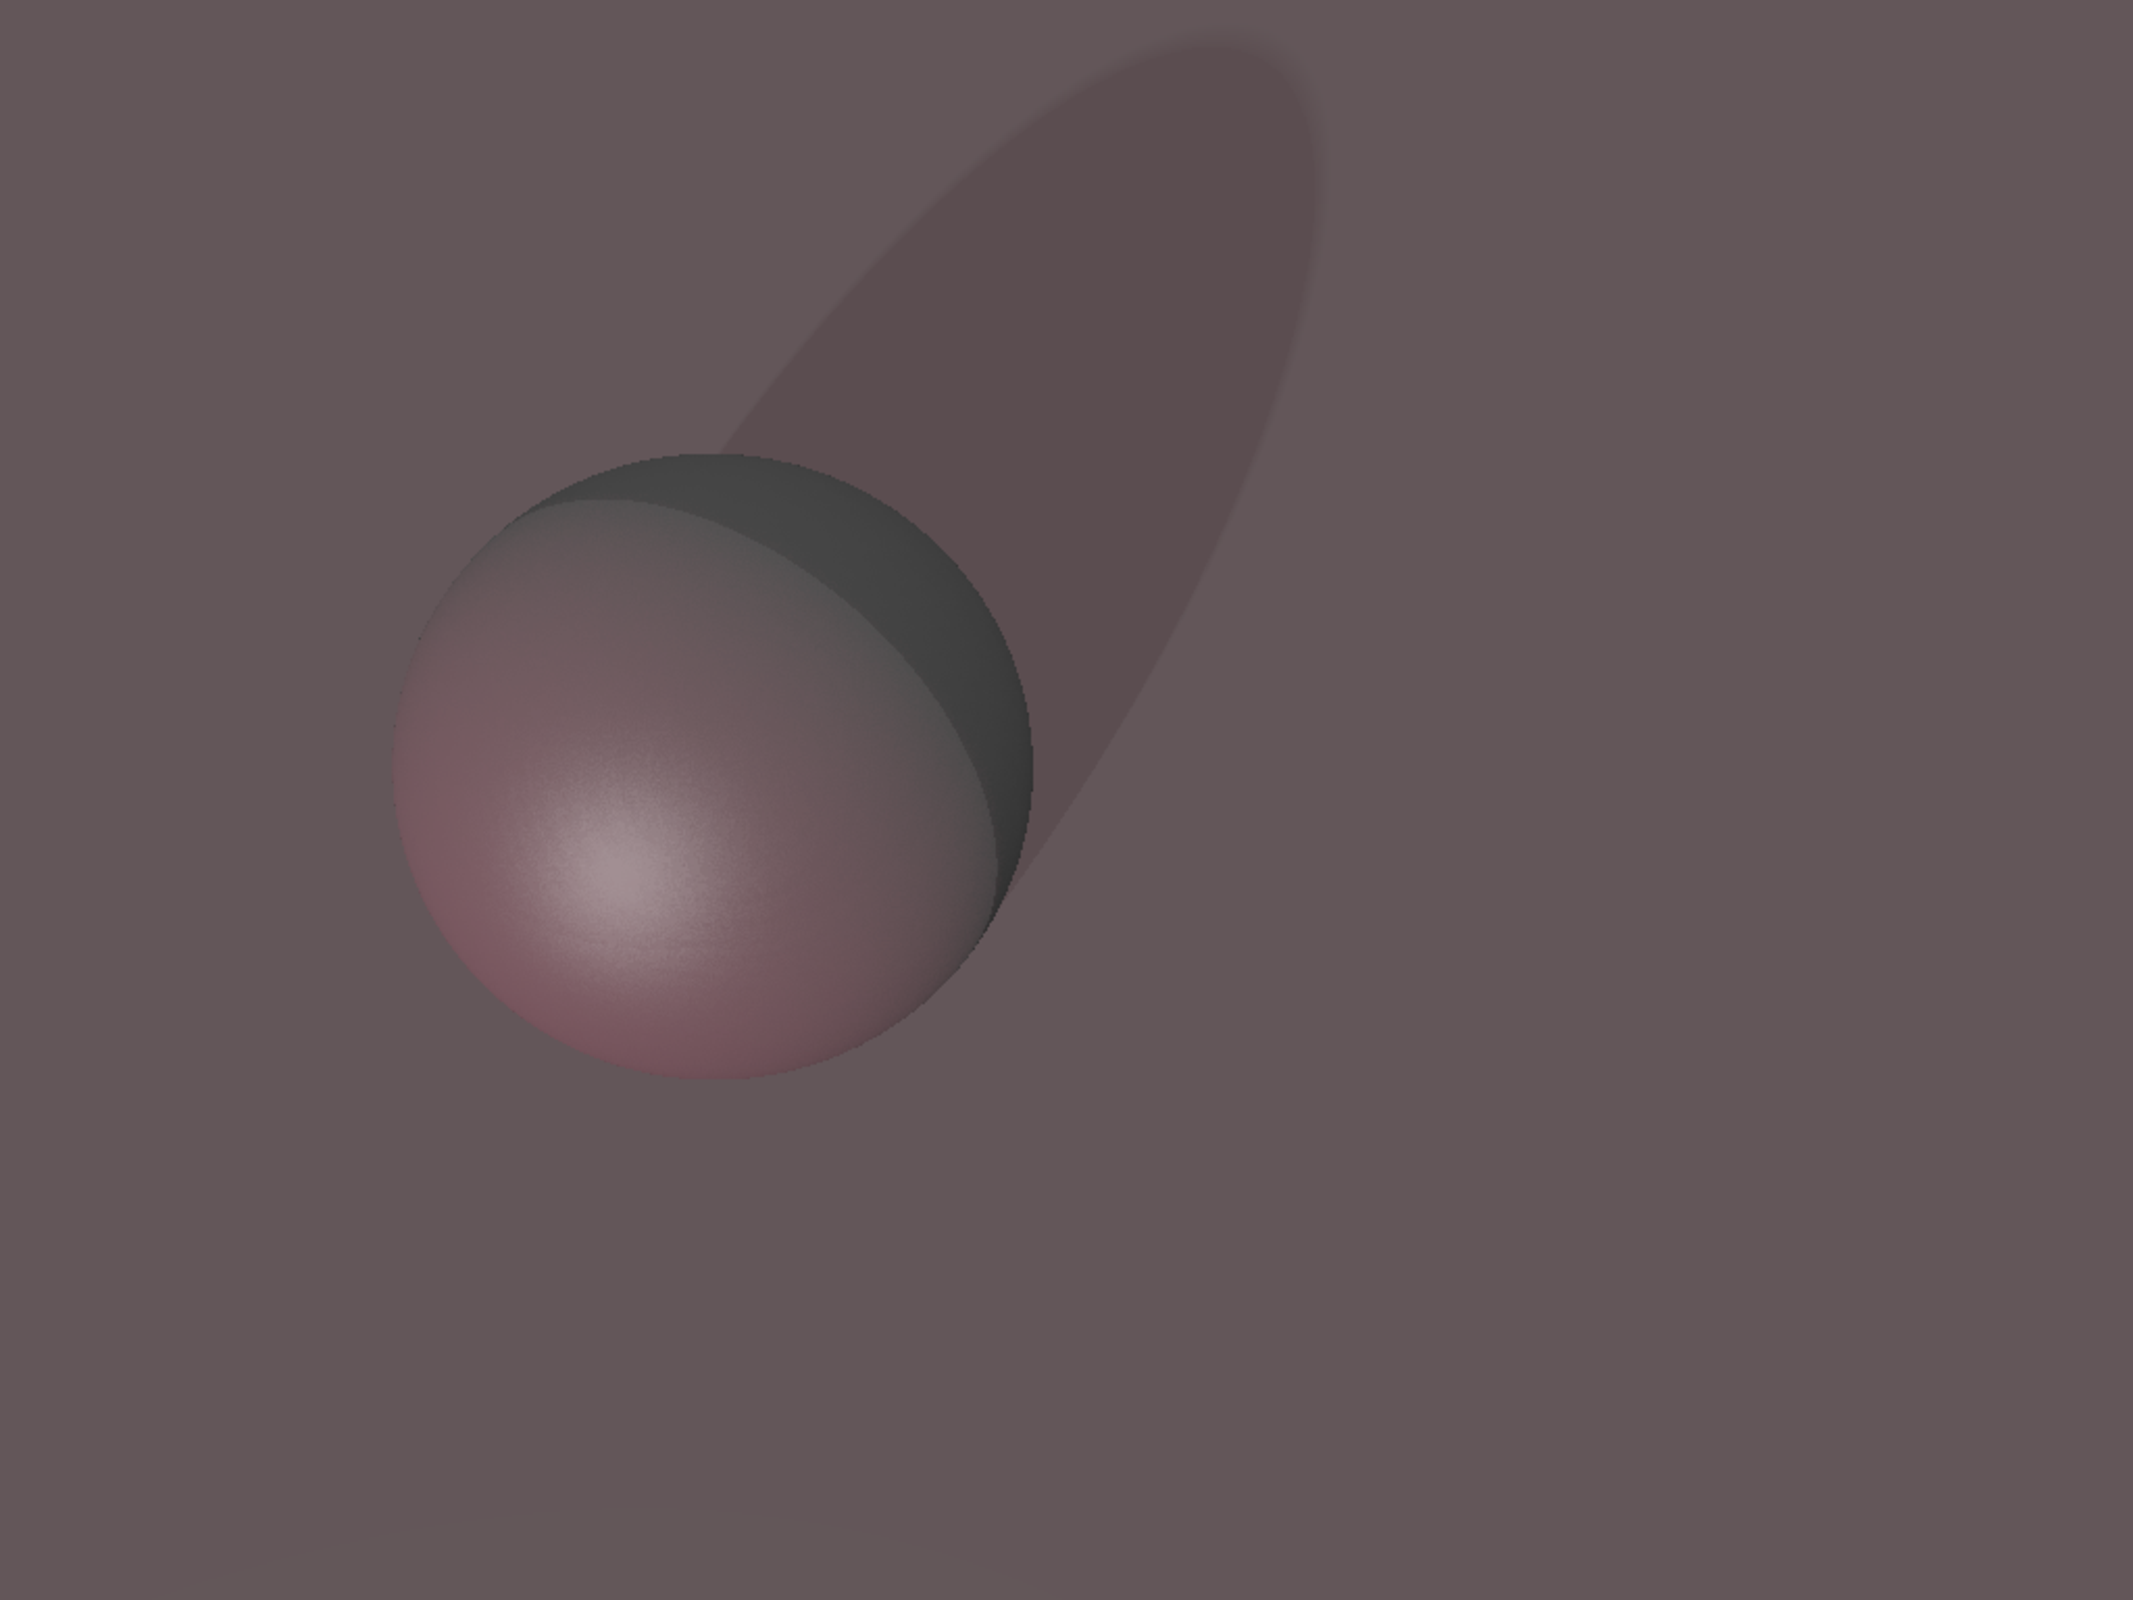
\includegraphics[width=0.3\textwidth]{img/sphere_tracing_shadows_64.pdf} \newline &
            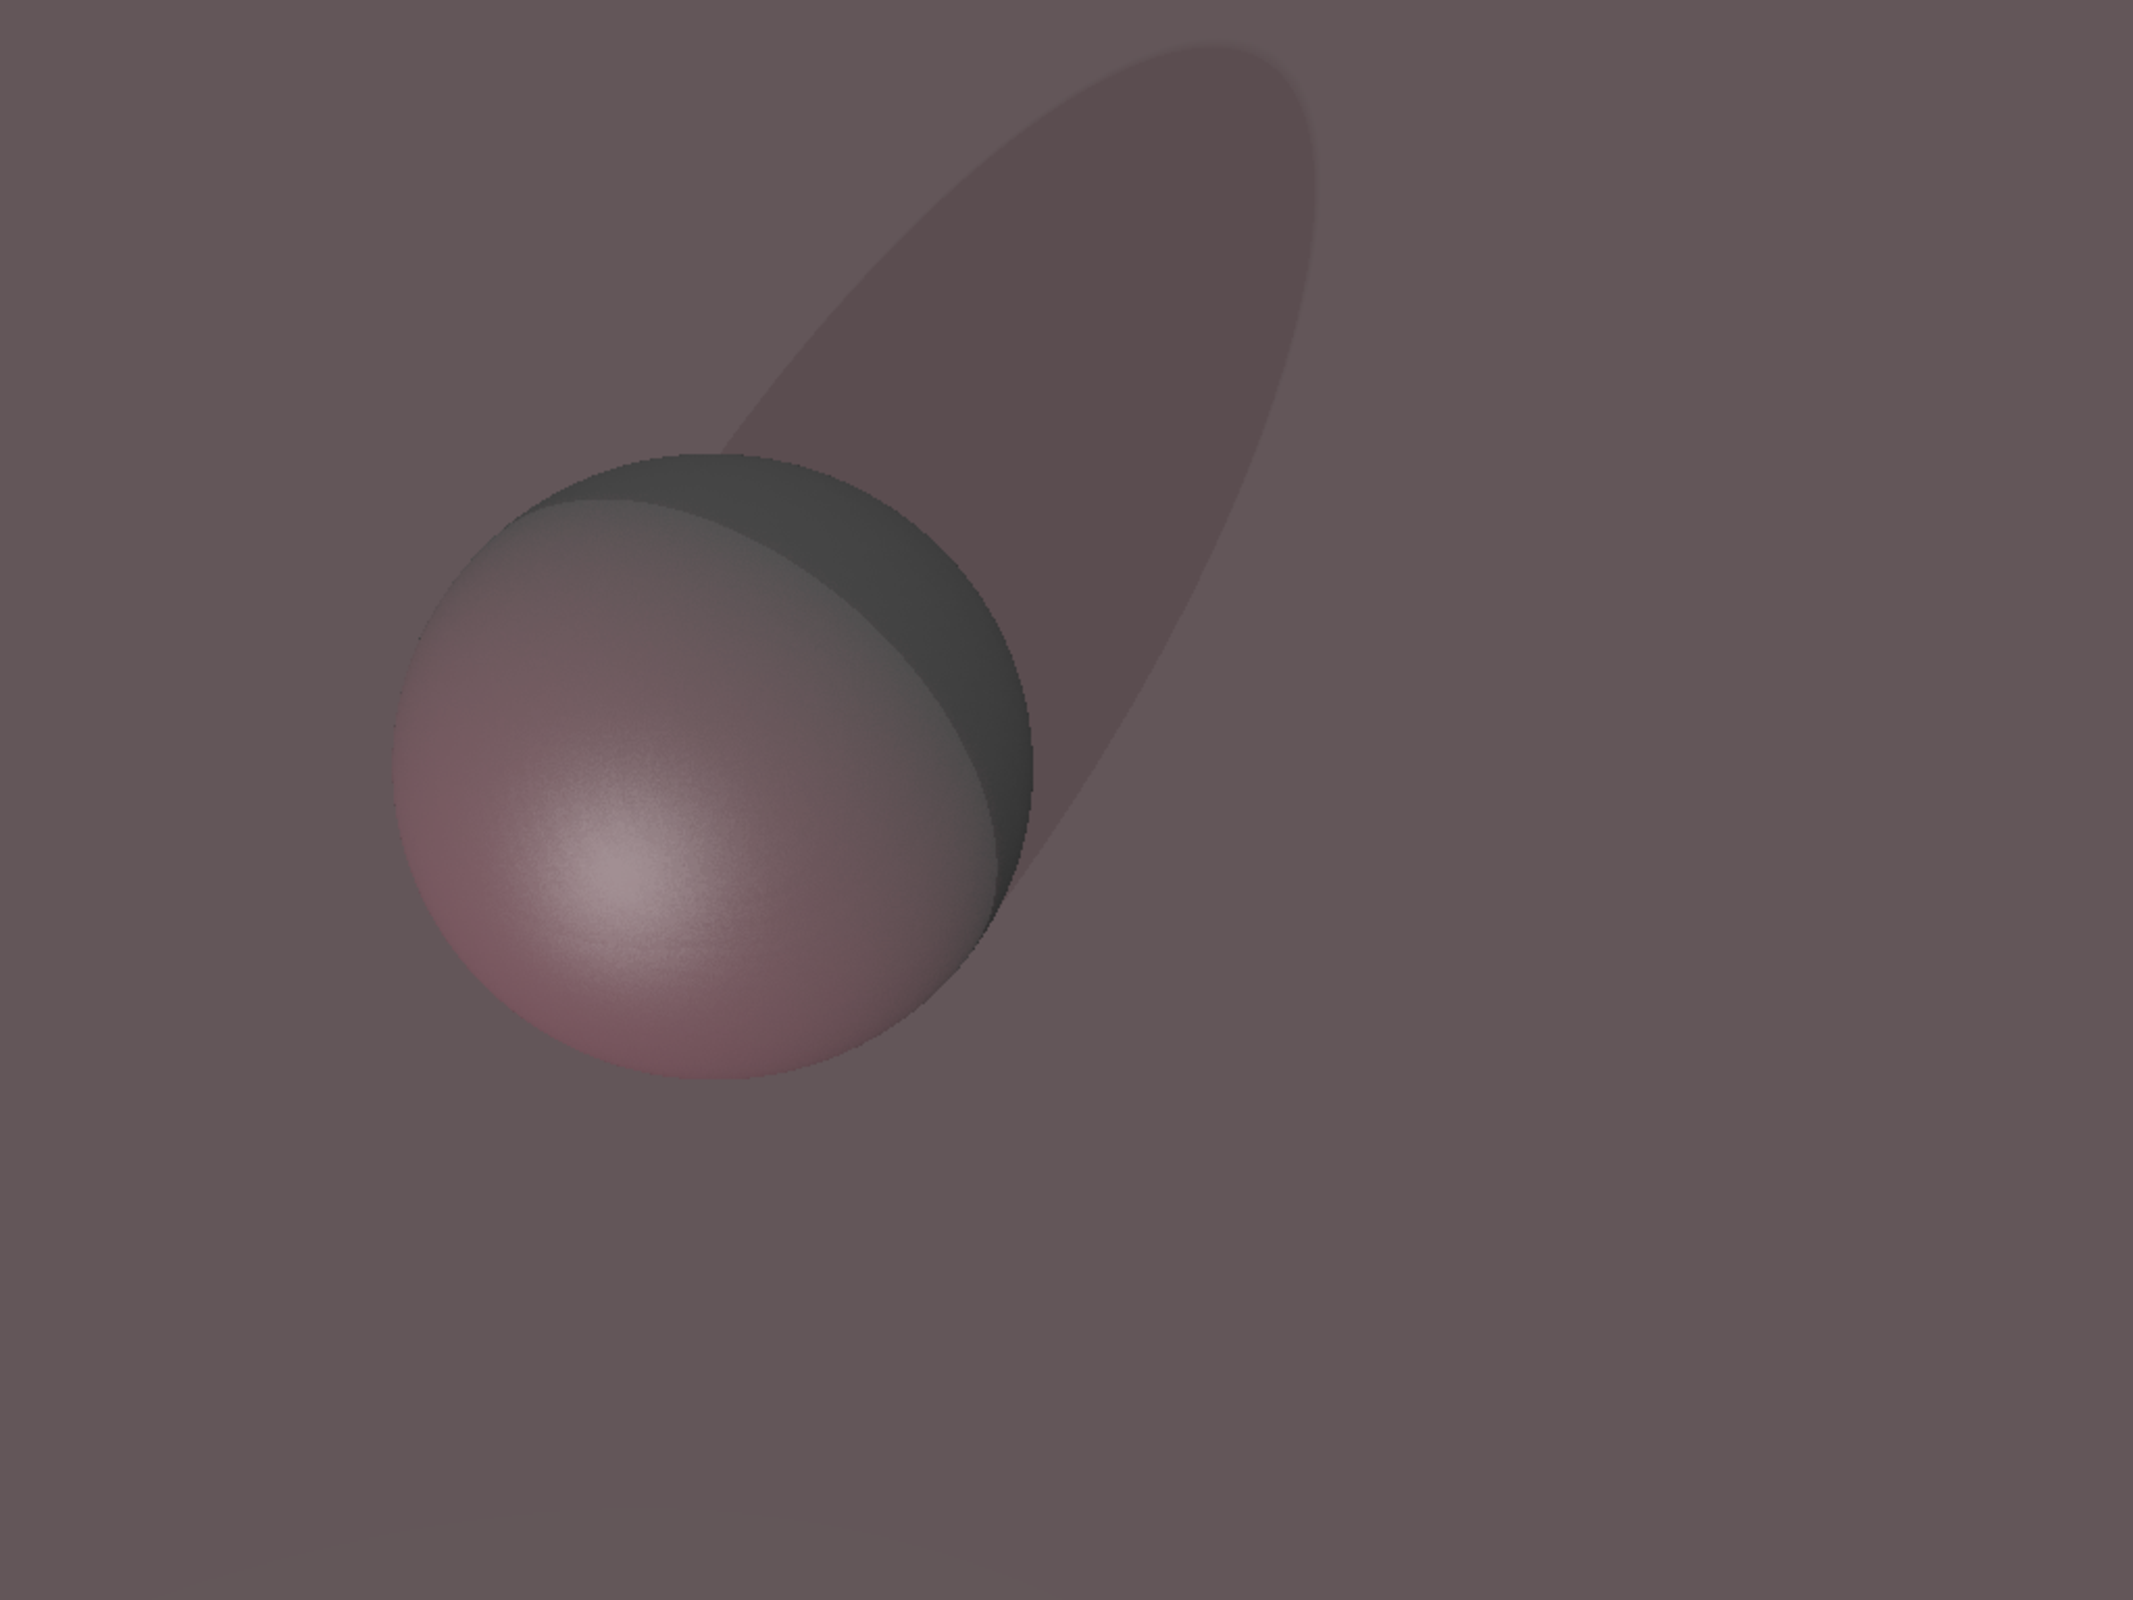
\includegraphics[width=0.3\textwidth]{img/sphere_tracing_shadows_128.pdf} \newline &
            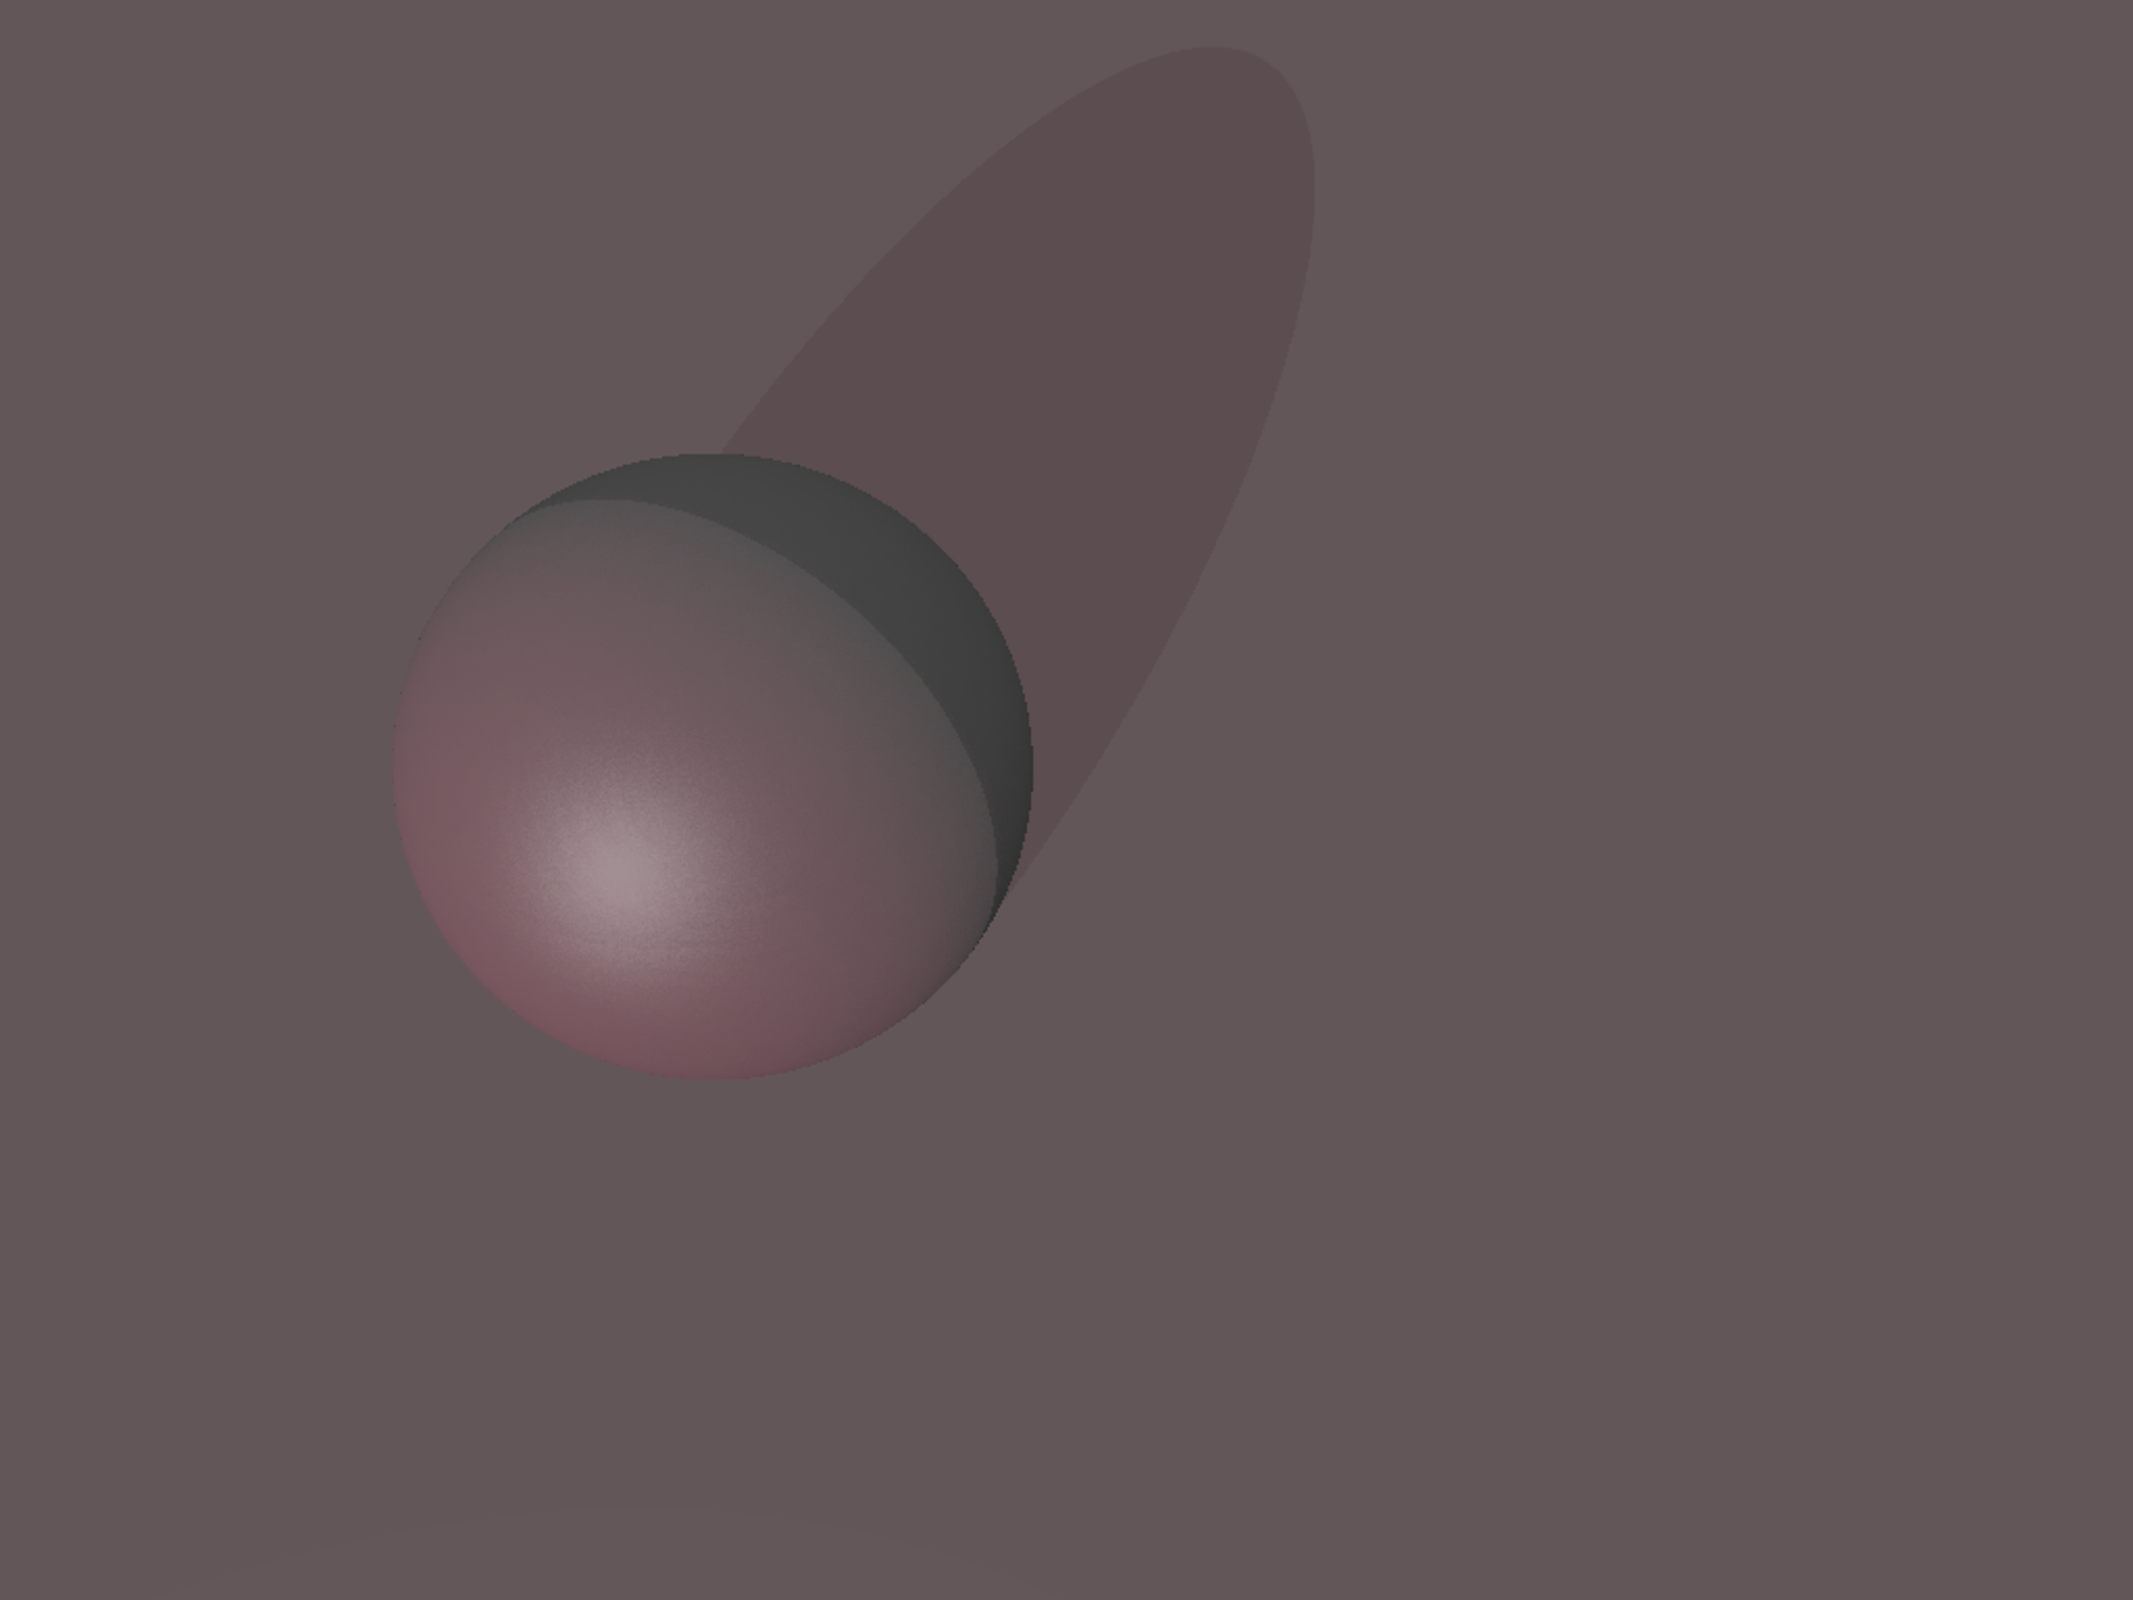
\includegraphics[width=0.3\textwidth]{img/sphere_tracing_shadows_256.pdf} \newline \\
        \bottomrule
    \end{tabular}
\end{table}

Das eigentliche Rendering, also die Darstellung der Szene, geschieht in
der Funktion \textit{render}.

\begin{lstlisting}[language=GLSL,caption={Funktion zur Darstellung der
        Szene in
        GLSL. Die Szene bzw.\ der Farbwert wird nur dann zurückgegeben
        bzw.\ berechnet, wenn eine minimale Distanz nicht unterschritten
        wird.},label={alg:glsl_render},captionpos=b,emph={render}]
// Performs rendering of a scene beginning at given origin in given ray
// direction. This invokes calculating the normal vector, the material
// as well as the lighting.
vec3 render(in vec3 rayOrigin, in vec3 rayDirection)
{
    vec3  color           = vec3(0.05, 0.08, 0.10);
    vec3  res             = castRay(rayOrigin, rayDirection, 100.0, 0.00001, 100);
    float currentDistance = res.x;
    float renderedScene   = res.z;
    float minimalDistance = -0.5;

    // Perform further calculation only when the distance is not below
    // the minimal distance (epsilon-factor).
    if (currentDistance > minimalDistance) {
        vec3 position = rayOrigin + currentDistance * rayDirection;
        vec3 normal   = calcNormal(position, 0.000001);

        vec3 lightColor    = vec3(0.7, 0.2, 0.3);
        vec3 lightPosition = vec3(-0.6, 0.7, -0.5);
        vec3 light         = calcLighting(position, normal, rayDirection, material, lightPosition, lightColor);

        color = light;
    }
    color      = clamp(color, 0.0, 1.0);

    return color;
}
\end{lstlisting}

Die Hauptfunktion \textit{main} des Fragment-Shaders ruft schliesslich
die Funktion zum Darstellen der Szene auf. Die zusätzlichen Methoden
(wie z.B.~\textit{getRay} oder~\textit{squareFrame}) finden sich
allesamt im Programmcode des Prototypen, welcher dieser Projektarbeit
beiliegt.

\begin{lstlisting}[language=GLSL,caption={Einstiegspunkt des
        Fragment-Shaders.},
    label={alg:glsl_main},captionpos=b,emph={main}]
// Main method of the shader.
void main()
{
    vec2 resolution      = globalResolution;
    float time           = globalTime * 1.1;
    float cameraAngle    = 1.0;
    float cameraHeight   = 2.0;
    float cameraPane     = 4.0;
    float cameraDistance = 4.5;
    vec3 rayOrigin      = vec3(cameraPane * sin(cameraAngle), cameraHeight, cameraDistance * cos(cameraAngle * time));
    vec3 rayTarget      = vec3(0.0, 0.0, 0.0);
    vec2 screenPosition = squareFrame(resolution);
    vec3 rayDirection   = getRay(rayOrigin, rayTarget, screenPosition, 2.0);

    vec3 color          = render(rayOrigin, rayDirection);
    color               = calcPostFx(color, screenPosition);

    gl_FragColor.rgb    = color;
    gl_FragColor.a      = 1.0;
}
\end{lstlisting}
